% Final Agescape manuscript, prepared 2026-11-07 for author preview only.
% PLOS ONE version, restructured 2026-11-08 from the Aging Cell copy: Materials and Methods moved
% after the Introduction (IMRaD order), Limitations kept as a subsection of the Discussion, Figure 6
% renumbered as Figure 5, Figures 5, 7, 8 remain Supporting Information S1 to S3, Ethics Statement
% and Data Availability with the AD Knowledge Portal acknowledgment added. Nothing submitted.
% Base: Rev1 Build B (19 pages) at repo head 7291470.
% The only commit since the Phase 0 to 3 head cb420de is 7291470, a CI pip cache fix with no new science.
% Nothing has been submitted, published, or pushed. Overleaf compile is a separate next step.
\documentclass[11pt]{article}

\usepackage[letterpaper,margin=2.2cm]{geometry}

\usepackage{graphicx}

\usepackage{booktabs}

\usepackage{longtable}

\usepackage{array}

\usepackage{hyperref}

\usepackage{caption}

\captionsetup{font=small}

\begin{document}

{\LARGE\bfseries Cell-type-specific compositional and transcriptional changes in mouse and human aging\par}\vspace{12pt}

Abolfazl Alipour


ORCID: 0000-0002-9757-8823


Correspondence: reza@kavoxlabs.com


Affiliation: [blank, pending author decision]


\section*{Abstract}

We tested whether aging is one universal mechanism, a single transcriptional program in every cell. Three hypotheses made the idea testable. H1: a mammalian methylation clock tracks age the same way across species. H2: the share of each cell type within an organ shifts in a conserved direction with age. H3: cells lose identity with age and transcribe more genes that do not belong to their program, so whole expression profiles drift away from young references in the same direction everywhere. None of the three behaved as a universal program. The clock reproduced, but it was not an independent validation, and it was far weaker in mouse than in human. Fractions shifted only in specific cell types in specific organs, clearest in human lung, and cross-species comparison showed neither conserved concordance nor conserved divergence. Cells did not consistently transcribe more off-program genes, and human profiles showed no overall drift, while mouse profiles did drift, spread across many cell types rather than driven by one. The durable human finding was narrower and targeted: specific genes changed reproducibly in interneurons across two cohorts, without general drift of their whole profiles. Gene-level changes shared direction across cell types more than chance allows, which shows coordination without a universal breakdown. Together these results rule out a single universal transcriptional program. Aging, at the level measured here, is not one mechanism: whatever the upstream causes are, they act through local, cell-type-specific routes, and any shared process must have consequences that differ by cell type.


\section*{Introduction}

Two views of aging predict different transcriptomes in old tissue. In the first view, one upstream failure drives the rest, so old cells of every type should show the same broad pattern: weakened identity, transcription of genes that do not belong to their program, and movement away from the young state in a shared direction. In the second view, aging is a label for several time associated processes that co occur and interact, with different weights in different tissues and cell types. That view predicts heterogeneity instead: some cell types change and others do not, directions differ, and no single pattern appears everywhere.


There is no agreed operational definition of aging in general. Intuitively, aging is loss of function after passage of time: tissues work less well as time passes, repair weakens, and the risk of disease and death rises. That intuition is not yet an operational definition, because it does not say what to measure. This paper therefore states its working operational definition plainly. In this study, aging is measured as three things: (a) cell-type fractions, the share of each cell type within an organ; (b) gene expression within specific cell types; and (c) the distance of a whole expression profile from a young reference. That is the paper's working definition for the analyses reported here, not a final word on aging itself. Any claim in this paper about aging is a claim about those three measurements, and any theory the paper constrains is constrained through them.


Bulk tissue measurements cannot separate these views, because a bulk change can reflect a shift in which cells are present rather than a change inside any cell. Single cell and single nucleus atlases allow composition and within cell expression to be measured separately, provided that sampling depth, detection differences between studies, reference choice, and the large number of cell type tests are handled as part of the inference rather than assumed away.


This study, Agescape, was designed around those separations. It asks whether a mouse derived transcriptional signature transports to human cohorts; whether the share of each cell type within an organ changes with age; whether complete expression profiles move away from young references; whether cells express more genes characteristic of other cell types as they age; and whether the targeted gene changes seen in human brain are global or specific. A formal concordance test, added in response to peer review, asks a narrower and answerable version of the universality question: do gene level age effects share direction across cell types within a tissue or cohort more than permuted age labels allow? Exploratory analyses in fruit fly, worm, zebrafish, and naked mole rat, a post hoc proliferation moderator analysis, and a published mammalian methylation clock benchmark are reported as supplementary material. They do not drive the title or the main claims.


The scope is stated at the outset. Every measurement here is transcriptomic, plus the methylation clock benchmark. Chromatin, DNA damage, transposon RNA, protein, cell function, and actual cell turnover were not measured. The results therefore test downstream transcriptomic predictions of mechanistic theories. They do not test the upstream mechanisms themselves, and no claim in this paper depends on pretending otherwise.


\section*{Materials and Methods}

\subsection*{Datasets and inferential units}

The mouse atlas was Tabula Muris Senis droplet data distributed through CZ CELLxGENE, with 23 mouse identifiers and 238,186 cleaned cells. Public human brain, kidney, and lung data came from the CZ CELLxGENE Census release of 2025-11-08, with 621 control donors for signature scoring and 479 cohort specific donors with adequate young reference coverage for expression vectors. The human lifespan cortex arm was the PsychAD dorsolateral prefrontal cortex lifespan atlas (Synapse syn52396927, with the pseudobulk resource syn62064518), with 284 control donors and 27 cell types. Exploratory arms were the naked mole rat skin data of Savina and colleagues (GEO GSE152886, five animals after exclusion of sample 2V), the Aging Fly Cell Atlas (GEO GSE218661, 36 age by sex pools in head and body), the Gao worm atlas (GEO GSE229022, 12 wild type pools), the Roux worm atlas (GEO GSE208154, descriptive only), and zebrafish testis (GEO GSE275361, ten males for broad compartments and six fish for fine grained analyses). Methylation benchmarks used GEO GSE199979 (339 mouse liver profiles) and GEO GSE184211 (661 human multi tissue profiles). Only primary, normal disease human cells were included, and public human analyses used donors aged at least 20 years. Donors, animals, fish, or pools were the inferential units, not individual cells. Depth is the total number of RNA molecules captured per cell, summarized as mean log UMI.


\subsection*{Mouse processing and differential expression}

Mouse cells were filtered using the prespecified atlas quality control rules: 500 to 5,000 detected genes, at least 1,000 UMIs, and doublet removal. Mitochondrial filtering was not applicable because the released droplet object lacked mitochondrial transcripts. Counts were normalized to 10,000 per cell and transformed with log1p. For differential expression, donor by cell type pseudobulk counts were aggregated and log transformed after counts per million scaling. Age effects were estimated within each cell type with sex included when identifiable. P values used t based regression inference and Benjamini-Hochberg correction within the stated family.


\subsection*{Signature derivation and transport}

P1\_Clean contained 139 mouse genes, 89 up and 50 down. P0\_Raw257 contained 257 genes and was retained as a sensitivity score. P1 used uniform Benjamini-Hochberg differential expression candidates from adequately covered mouse units and removed predicted or pseudogene labels, non protein coding biotypes, ribosomal and mitochondrial genes, and specified ambient RNA cases. Sex dimorphic and immediate early filters belonged to P2 and P3, not P1. One to one mouse to human orthologs came from the committed Ensembl derived mapping, giving 118 mapped P1 genes. The score was mean expression of up regulated genes minus mean expression of down regulated genes, with missing genes omitted rather than imputed. Public cohort regressions included age and sex when variable. Primary PsychAD models included age, sex, brain bank, postmortem interval, and three technical principal components. One Benjamini-Hochberg family covered 225 public cohort cell type tests and 27 primary PsychAD tests, for 252 tests. The matched null analysis in PsychAD generated 200 random signatures per cell type, each matching the detected P1 up and down counts and expression decile distribution, excluding P1 genes from the candidate pool, and using the same score and fully adjusted regression.


\subsection*{Cell type composition}

A cell fraction is the share of one specific cell type among recovered cells in one organ, modeled as a centered log ratio slope. A fraction is never a tally across different denominators, never an absolute cell count, and a change in a fraction is not by itself evidence of fibrosis or of organ damage.

For donor i and cell type j, counts were transformed with pseudocount a and the centered log ratio: CLR\_ij = log((count\_ij + a) / sum\_j(count\_ij + a)) minus the mean over j of the same logged shares. The primary pseudocount was 0.5. Primary regressions included age and sex when identifiable. Reviewer response models added log total recovered cells and evaluated pseudocounts 0.1, 0.5, and 1.0, and a global Benjamini-Hochberg recheck applied one correction across the core mouse, human, and naked mole rat tests. Propeller provided a donor level count model check: proportions were transformed as logit((count + 0.5) / rowSum(count + 0.5)), followed by limma empirical Bayes regression with age, log total cells, sex when variable, and platform for Gao worm. Recovered composition was not interpreted as absolute tissue cell number.


\subsection*{Whole expression vector displacement}

An expression vector is a complete within-cell expression proportion vector. No UMI downsampling was used for the direct vector analysis. Mitochondrial, ribosomal, and sex linked marker genes were excluded using species appropriate symbols. Each cell raw count vector was converted to within cell proportions p, and a young reference probability vector q was constructed from pooled counts of the same annotated cell type, with young donors or animals excluded from their own reference. Hellinger distance was H(p,q) = sqrt(1 minus sum over g of sqrt(p\_g q\_g)). Each evaluated donor by cell type unit required at least 20 cells and at least 50 remaining young reference cells. Mouse young references used animals aged 1 or 3 months, and human references used donors aged 20 to 40 years. Continuous age models included sex and, in specified arms, mean log UMI. Species summaries used unit fixed intercepts and donor clustered standard errors. Effects were scaled to 10 percent of species maximum lifespan using AnAge values of 4 years for mouse, 122.5 years for human, and 31 years for naked mole rat. The mouse leave one cell type out analysis removed each cell type across all tissues and refit the global model.


\subsection*{Gene effect concordance across cell types}

Donor pseudobulk counts were aggregated per cell type, normalized to counts per 10,000, and log1p transformed. Each cell type yielded a vector of gene level age effects from models including age, sex when variable, mean log UMI, and platform for Gao worm. Pairwise Pearson and Spearman correlations were computed between cell type effect vectors within a tissue or cohort, and the primary summary was mean pairwise Pearson correlation. Age labels were permuted within cell type while preserving sex and platform strata, with 200 permutations, except naked mole rat, which used all ten assignments of two aged animals among five. A random effects meta analysis combined the six global Hellinger estimates using inverse variance weighting and a DerSimonian-Laird residual heterogeneity estimate, with the worm day 6 reference as primary and day 1 as sensitivity.


\subsection*{Off program expression, entropy, and depth sensitivity}

Off program expression means expression of genes that are uncommon in young cells of the target type but characteristic of another cell type. That outcome is never called entropy in this paper. A separate Shannon entropy measure is reported under its own name where it was computed.

Within cell Shannon entropy was minus the sum over g of p\_g log(p\_g), after the stated gene exclusions. Off program genes were uncommon in young target cells but characteristic of another lung cell type: detection in at most 5 percent of young target cells and at least 20 percent of another cell type, expression of at least 20 counts per 10,000, and at least fivefold enrichment over the target. Young references excluded the evaluated young animal. Animal means were regressed on age and sex with Benjamini-Hochberg correction across cell types. The original analysis downsampled all cells without replacement to 1,500 UMIs. Reviewer response analyses evaluated 500, 1,500, and 3,000 UMIs and full depth, with no downsampling in the full depth arm, the original 1,500 UMI inclusion threshold retained, young reference marker definitions fixed across depths, and off program fractions computed against actual total UMIs. The library size arm added each animal mean log actual pre downsampling depth. Global models used cell type intercepts and animal clustered t based inference.


\subsection*{Human nonlinear age models and annotation stability}

Nonlinear age effects used a cubic B spline with three degrees of freedom, fixed before examining results. F tests compared nonlinear and linear models on the same donor by cell type units, with Benjamini-Hochberg correction within cohort separately for linear and nonlinear comparisons. For annotation stability, excluded and unassigned cells were tabulated by age and tissue or cohort, and Spearman tests assessed age associations of excluded and unassigned fractions. A fixed canonical marker panel was evaluated by donor by cell type log counts per 10,000 expression with age, sex, and depth covariates, requiring at least six donors and 20 cells per donor by cell type unit, with Benjamini-Hochberg correction across targeted marker tests. Marker change was not equated with identity loss.


\subsection*{Bayesian hierarchical models}

Bayesian disorder and vector outcomes were standardized within cell type. Models used global effects, non centered cell type intercepts and age slopes, animal or donor intercepts, cell type residual scales, and Student t residuals. The primary global age prior was Normal(0, 0.5), with prior standard deviations of 0.25 and 1.0 as sensitivity analyses. Posterior means, 94 percent highest density intervals, and probabilities of a positive effect were reported, with prior predictive, convergence, posterior predictive, calibration, and influential observation diagnostics retained. Bayesian estimates were exploratory when cohorts were small or diagnostics warned.


\subsection*{Methylation benchmark}

Published Universal Clock 2 coefficients were applied without refitting. Chronological age was scaled using species maximum lifespan and gestation time, and the published inverse link correction was applied. Mouse scoring used 724 of 816 clock probes present in the array file. Per sample predictions were saved. Predictive R squared was 1 minus SSE/SST on chronological age predictions, distinct from squared Pearson correlation, and mean absolute error and correlations were reported separately. Neither evaluation was presented as independent validation.


\subsection*{Reproducibility and reporting}

Aggregate result tables were committed for every reported number, and the Evidence and Caveats appendix traces each key number to its committed result file. Controlled PsychAD donor level values and identifiers were not exported. Exploratory, secondary, and primary families were labeled explicitly. Non significance was not treated as equivalence unless a stated equivalence test supported it.


\section*{Results}

\subsection*{Cell fractions change locally, in specific types and organs}

Fraction changes (the share of one specific cell type among recovered cells in one organ, modeled as a centered log ratio slope) were found in some organs and datasets and not in others, and always in specific cell types. Because the first draft corrected composition tests within each organ or cohort, the reviewer response re ran one Benjamini-Hochberg family across the core mouse, human, and naked mole rat composition tests. Under that wider family, mouse retained at least one significant fraction change in seven organs, down from eight, and tongue no longer qualified. Human data retained at least one change in two cohort datasets, down from three, and Kidney Living Donor no longer qualified. MSSM retained three changes and integrated lung retained two under the global correction (Figure 1).


The human lung gives the clearest named example. In the integrated lung cohort, 119 donors and 44 cell types, club cells decline with age (slope minus 0.060227, q = 0.004423) and multiciliated epithelial cells decline with age (slope minus 0.034154, q = 0.022513). Under the wider global correction across the core mouse, human, and naked mole rat tests, both remain significant, with q = 0.0053 for club cells and q = 0.0248 for multiciliated epithelial cells. These are fraction changes among recovered cells in one organ, not measurements of absolute cell number, fibrosis, or organ damage.


Three sensitivity analyses support reading these as fraction changes among recovered cells, and nothing more. Models adjusted for log total recovered cells gave, within their own strata, 15 significant mouse tests across six organs and ten human tests across three cohort datasets. Pseudocounts of 0.1, 0.5, and 1.0 gave strongly correlated effects: the correlation between the 0.1 and 1.0 arms was 0.9569 in mouse and 0.9434 in human, and the share of tests with the same sign in all three arms was 0.9412 in mouse and 0.9313 in human. A propeller logit plus limma check agreed closely with the centered log ratio models, with Spearman rho of 0.9738 in mouse and 0.9313 in human, and with ten mouse and nine human results passing false discovery rate correction in both models. These models change some individual significance calls. They do not turn recovered cell counts into direct measurements of absolute tissue composition, and no fraction result in this paper demonstrates fibrosis or organ destruction.


\begin{figure}[htbp]\centering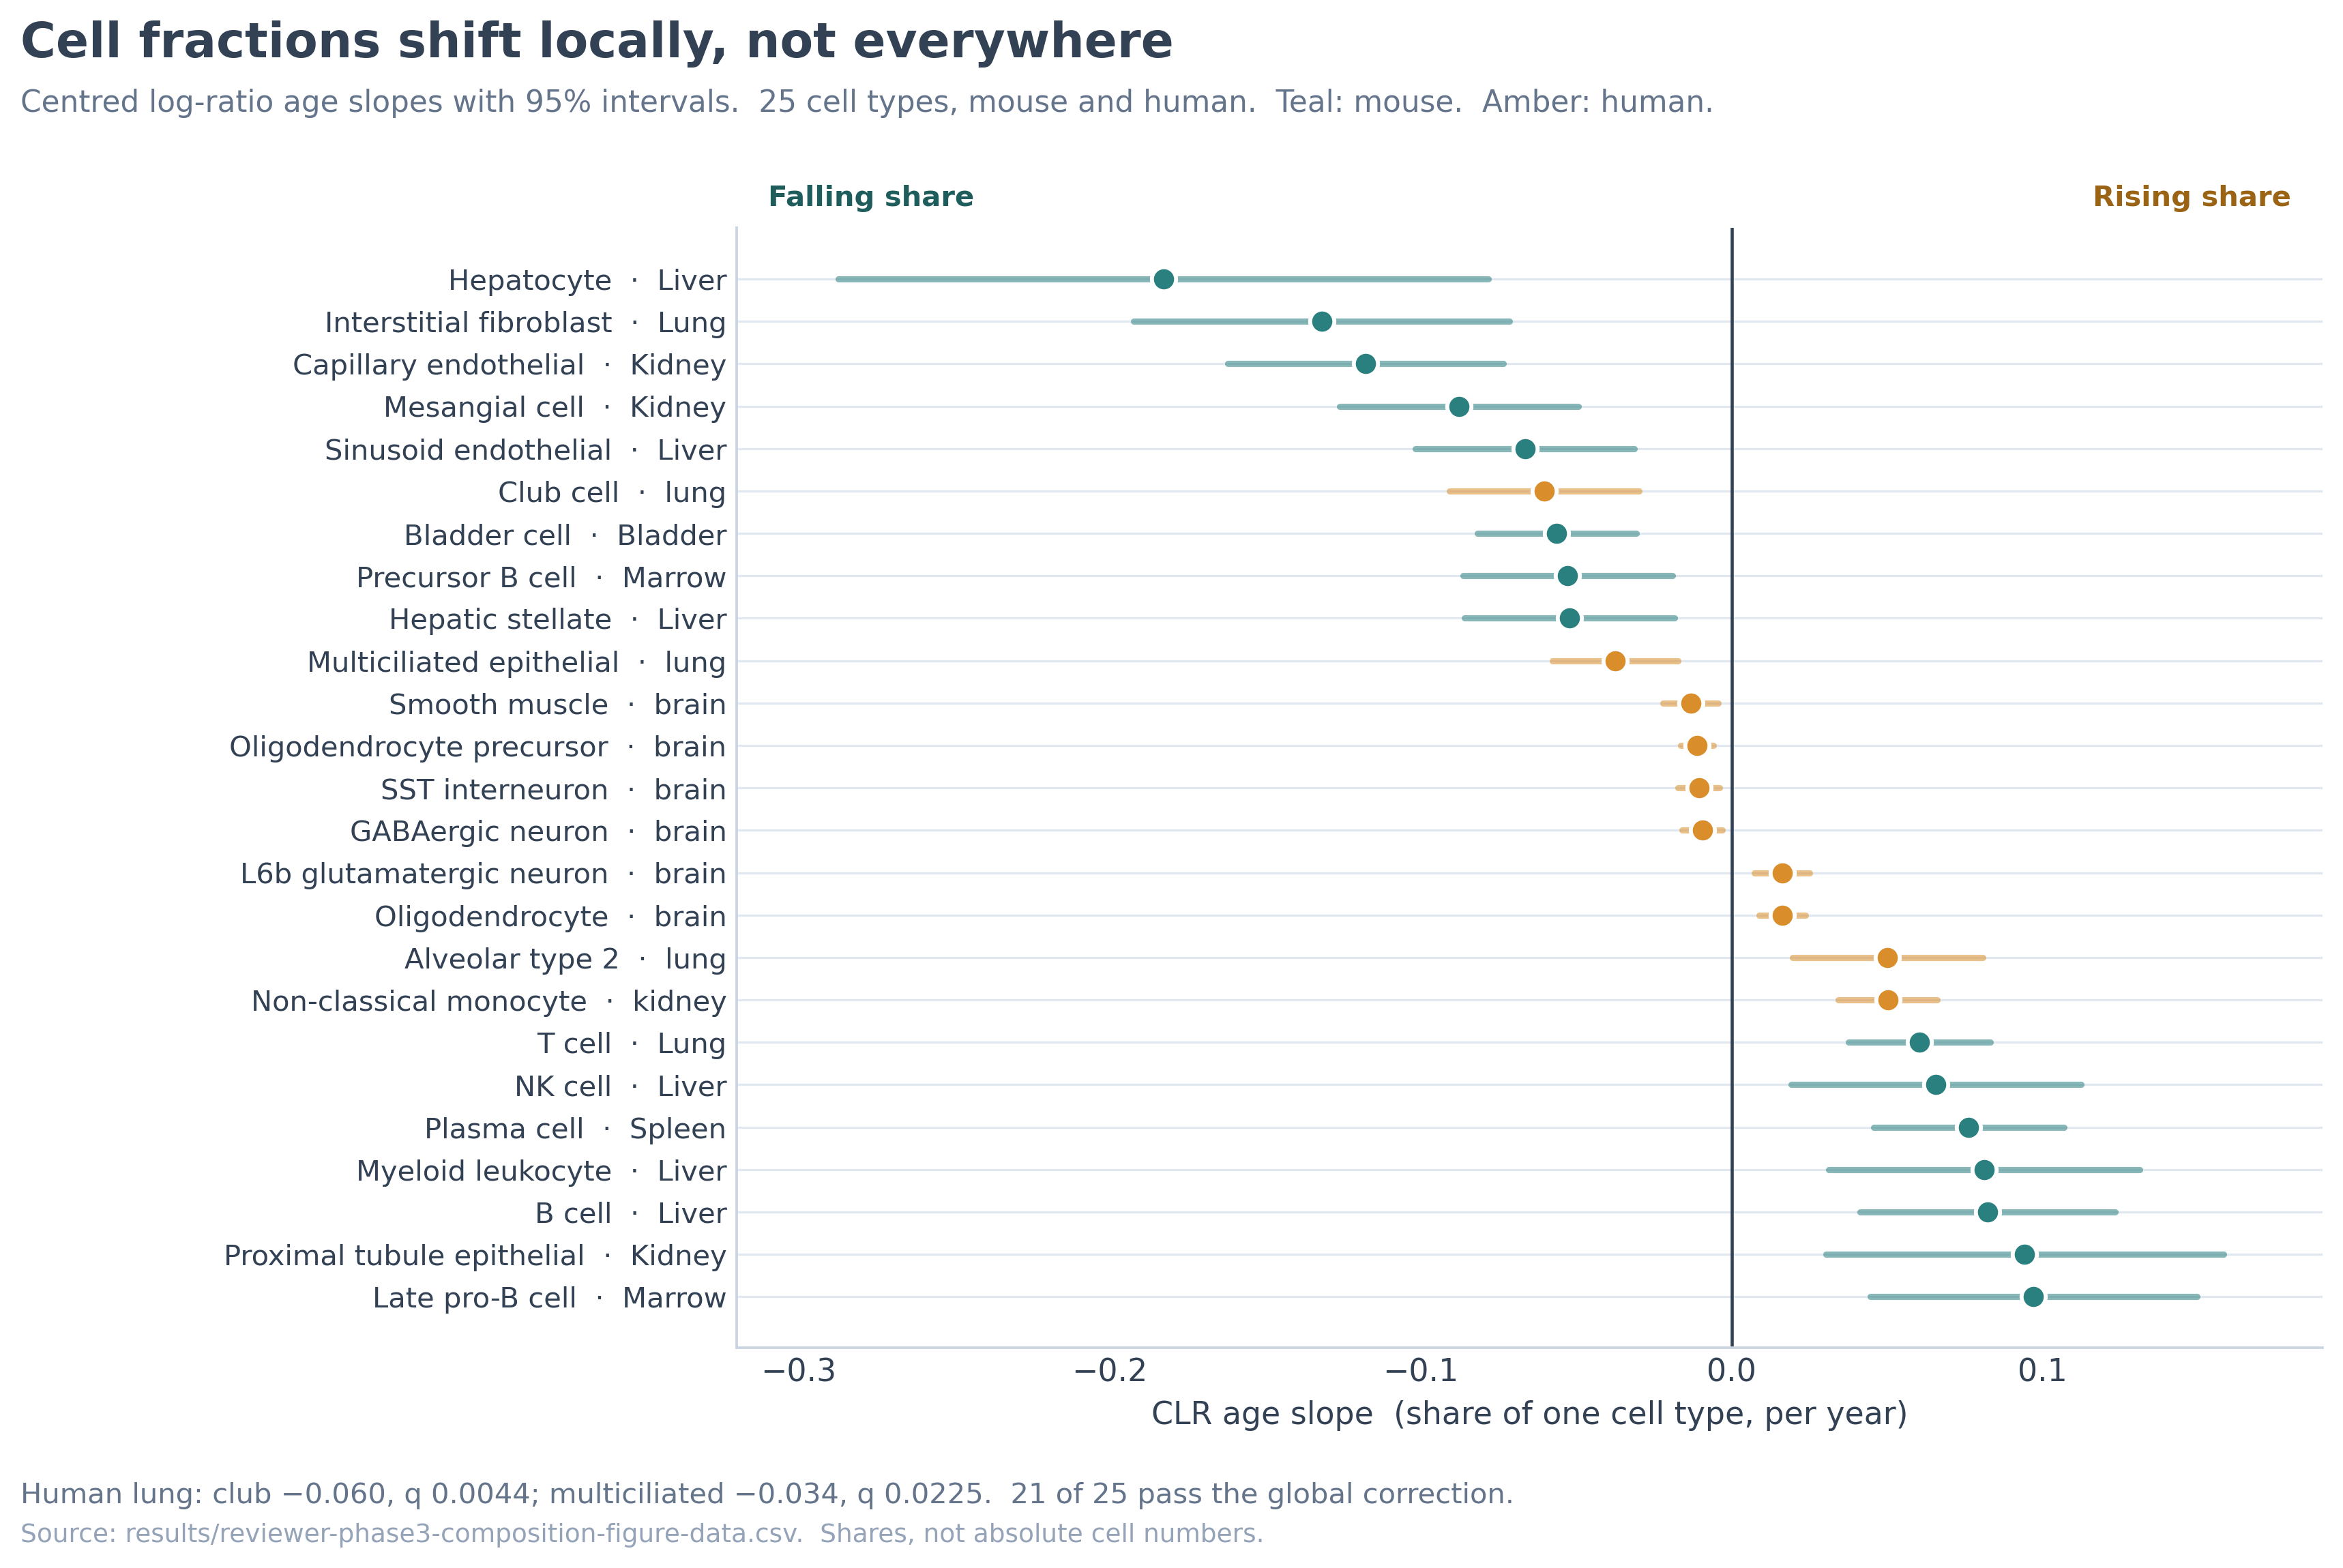
\includegraphics[width=0.92\textwidth,height=0.42\textheight,keepaspectratio]{figures-v2/fig1-composition.png}\caption{Figure 1. Composition changes with confidence intervals. Points are mouse or human cell fraction age slopes after adjustment for log total recovered cells, sex when identifiable, and the fixed 0.5 pseudocount. Bars are 95 percent confidence intervals. 21 of the 25 shown pass the global correction. The outcome is the centered log ratio share among recovered annotated cells. The figure does not measure absolute tissue cell numbers, prove fibrosis, or eliminate age related recovery and annotation biases. Data: results/reviewer-phase3-composition-figure-data.csv.}\end{figure}

\subsection*{A mouse derived signature transports only to specific human cell types, and not beyond matched random signatures in PsychAD}

The primary signature, P1, contains 139 mouse derived genes, 89 up regulated and 50 down regulated with age, after technical and biotype filtering. The 257 gene P0 signature is a sensitivity analysis only. P1 was derived from the mouse differential expression analysis before the reported human transport evaluations, and no human result was used to choose its membership. One to one mouse to human mapping yields 118 genes, 76 up and 42 down, with missing genes omitted rather than imputed.


Across 252 primary human cell type tests under one shared correction, only three survived: MSSM layer 2/3 neurons, MSSM oligodendrocytes, and PsychAD EN\_L3\_5\_IT\_3 neurons. Re correction of the same 252 p values without outcome based deletion left the three survivors and their q values unchanged. Whole cortex transport was not detected. No oligodendrocyte precursor cell or microglial result survived the primary correction, so those results remain candidates, not established findings.


Two qualifications now bound this result. First, PsychAD is not independent replication of the public cohorts. Exact identifier matching established that 103 of 214 public MSSM donors and 131 of 134 public HBCC donors also appear in the corresponding PsychAD brain bank arms, with concordant age and sex. The MSSM to HBCC interneuron comparison below uses different source banks and is not reclassified by this overlap. Second, a matched random signature analysis in PsychAD generated 200 expression decile matched random signatures per cell type, using the same score and the fully adjusted model. No PsychAD cell type survived Benjamini-Hochberg correction against this null; the smallest q value was 0.1007. Within PsychAD, the reported P1 associations should therefore be treated as not distinguishable from expression matched random signatures under this test. The null was run in PsychAD only, not across every public cohort.


\subsection*{Mouse whole profile displacement is distributed, and the human overall displacement is small}

Mouse showed a robust global vector signal (an expression vector is a complete within-cell expression proportion vector, compared by Hellinger distance to a cross-fitted young reference from the same cell type, with no per-cell downsampling): plus 0.1028 standard deviations per 10 percent of maximum lifespan (p = 0.00000398), and it survived depth adjustment (depth is the total number of RNA molecules captured per cell, summarized as mean log UMI). A decomposition added in response to review shows that this signal is not one cell type in disguise. Forty five of 62 mouse tissue by cell type units had positive unadjusted Hellinger age slopes, with an exact sign test p = 0.000497. Leave one cell type out global effects ranged from plus 0.0970 to plus 0.1119 around the full estimate of plus 0.1028, and the largest absolute change from removing any one cell type was 0.00912 standard deviations. The largest reductions followed removal of mesenchymal stem cells, podocytes, fenestrated cells, lung fibroblasts, or endothelial cells. No single cell type removes the global association (Figure 2).


The human overall vector effect was plus 0.0365 standard deviations (p = 0.2218), with a 95 percent confidence interval of minus 0.0221 to plus 0.0951. Unlike the other nulls in this paper, this one was precise enough to support an equivalence statement at a stated margin: the minimum detectable effect at 80 percent power was 0.0837 standard deviations, and equivalence was established at both the 0.1 standard deviation margin (p = 0.0169) and the 0.25 standard deviation margin. That is a statement about the overall human displacement averaged across units. It does not exclude local displacement in specific cell types, and the targeted interneuron result below is exactly such a local case.


\begin{figure}[htbp]\centering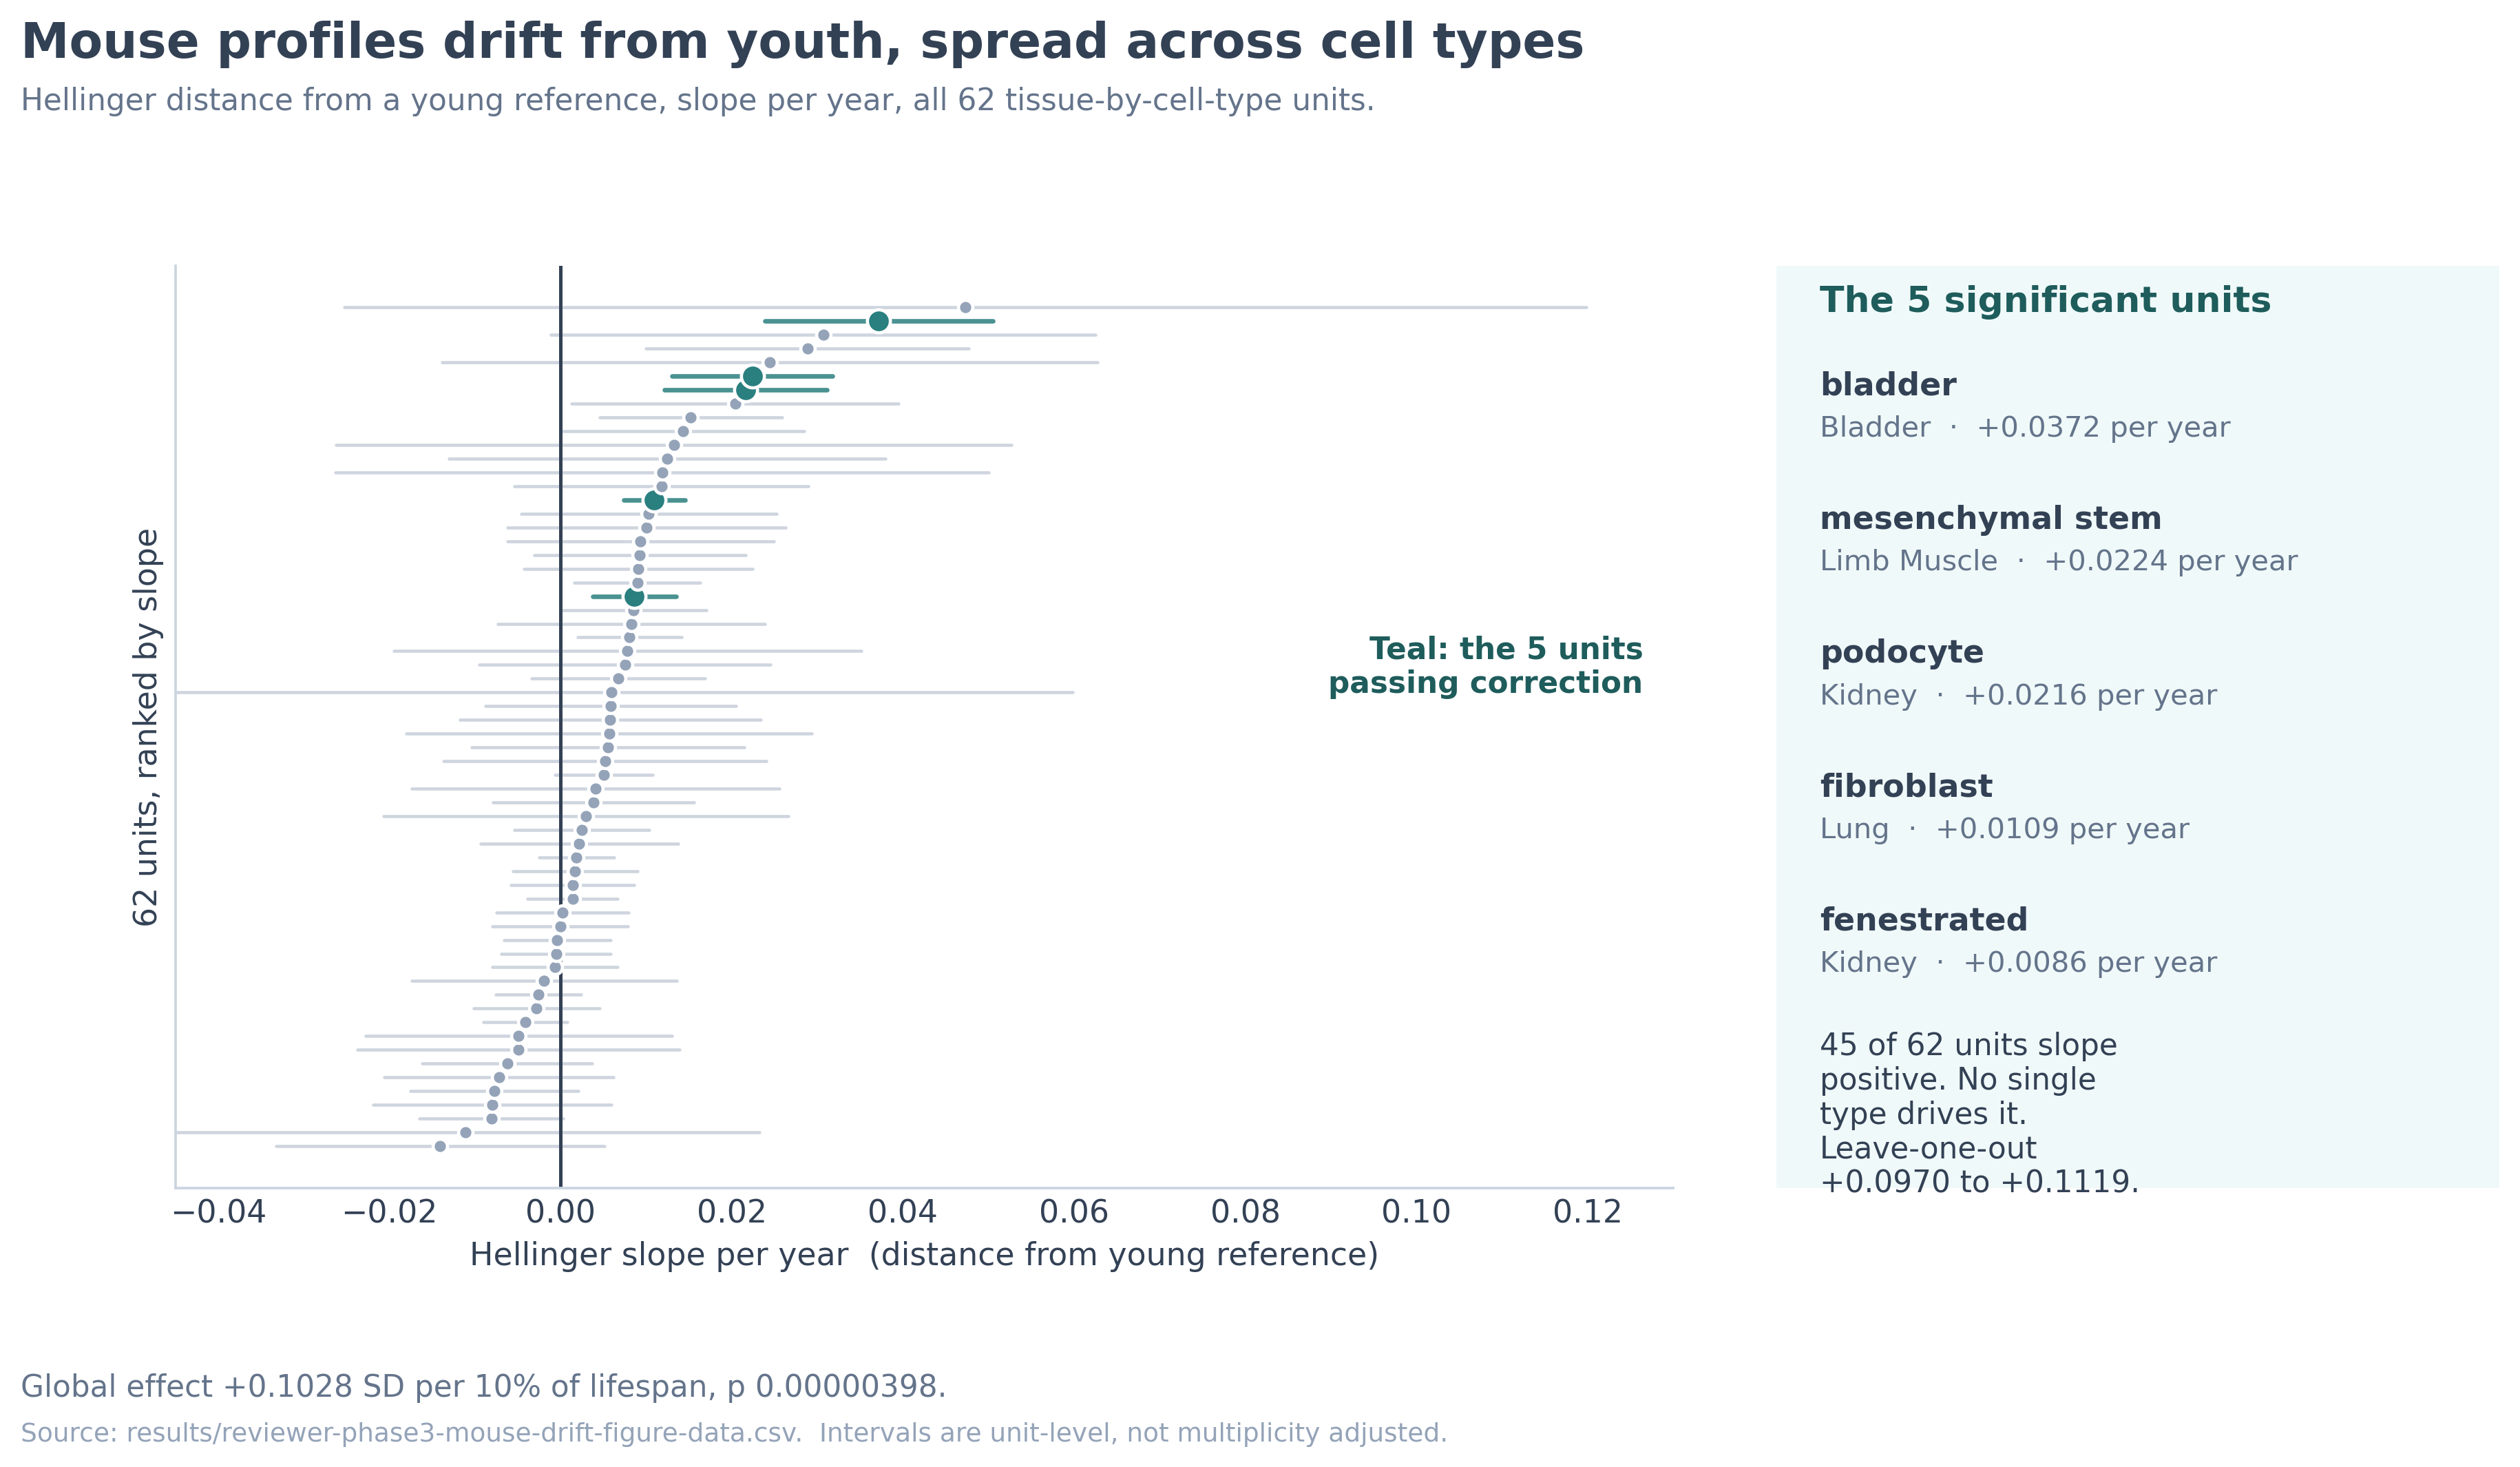
\includegraphics[width=0.92\textwidth,height=0.42\textheight,keepaspectratio]{figures-v2/fig2-mouse-drift.png}\caption{Figure 2. Mouse vector drift by cell type. Each point is a donor level age slope in mean Hellinger distance from a cross fitted young expression reference for one mouse tissue by cell type unit, ranked by slope; all 62 units are shown. Bars are 95 percent confidence intervals. Teal points are the five units passing correction, listed in the side panel. Positive values indicate increasing distance from the young reference. The figure does not show increased random noise, DNA damage, or a universal aging program, and it does not adjust the displayed unit level intervals for multiplicity. Data: results/reviewer-phase3-mouse-drift-figure-data.csv.}\end{figure}

\subsection*{Gene level age effects share direction across cell types, without establishing a universal program}

The concordance test compares gene level age effect vectors between cell types within a tissue or cohort, with age labels permuted within cell type while preserving sex and platform strata. In mouse, mean pairwise Pearson concordance was plus 0.1804, against a permutation null mean of plus 0.0011 with a null 95 percent interval of minus 0.0113 to plus 0.0180 (permutation p = 0.004975). In human, mean pairwise Pearson concordance was plus 0.1981, against a null mean of minus 0.0003 with a null interval of minus 0.0067 to plus 0.0092 (permutation p = 0.004975). Gene level effects therefore share direction across cell types more than chance allows in both main species (Figure 3).


This result cuts in a specific direction and no further. Shared direction of gene level effects is not evidence that every gene changes, that whole vector distance increases everywhere, that transcriptional disorder increases, or that the same genes respond across species. A random effects meta analysis of the global Hellinger effects across all six species, using the balanced worm day 6 reference, gave a pooled effect of plus 0.0721 standard deviations per species specific age scale, with a 95 percent confidence interval of minus 0.0232 to plus 0.1674 (p = 0.1383) and substantial heterogeneity (Q = 15.20 on 5 degrees of freedom, p = 0.00956). With the worm day 1 reference the pooled effect was plus 0.1454 (95 percent confidence interval minus 0.0182 to plus 0.3090, p = 0.0815). The cross species average is therefore not a stable universal effect, while within species gene level concordance is real. Both statements are needed, and neither cancels the other.


\begin{figure}[htbp]\centering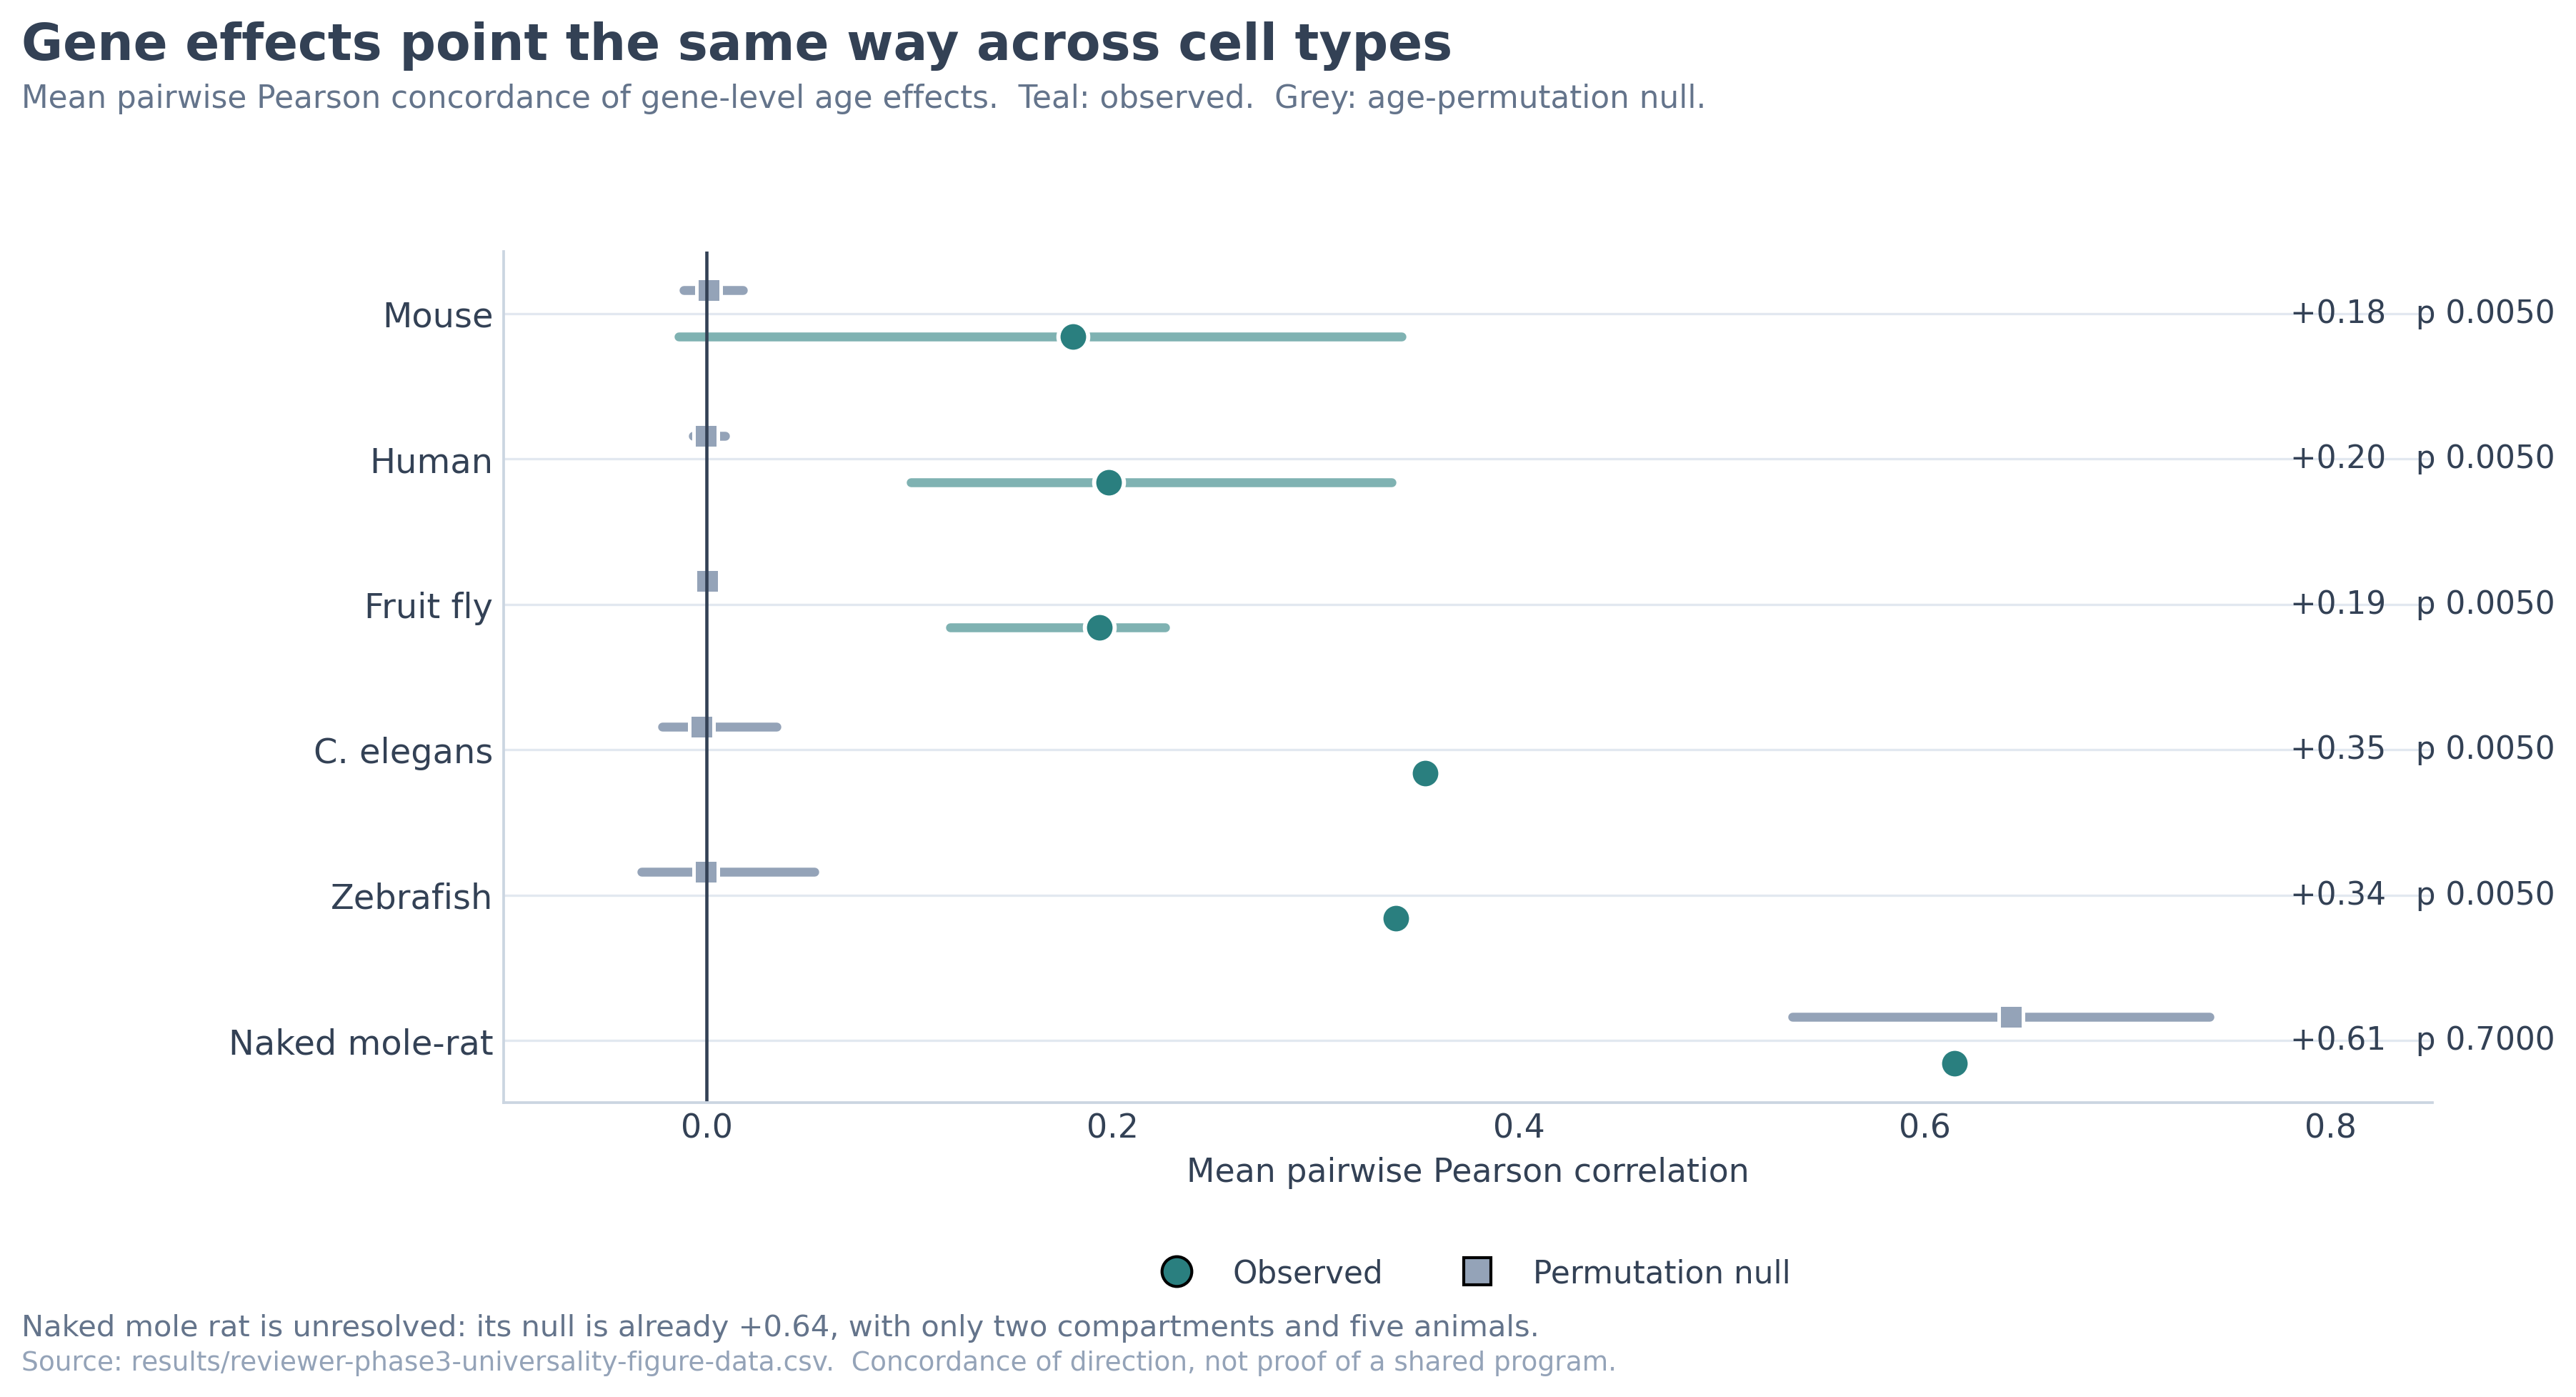
\includegraphics[width=0.92\textwidth,height=0.42\textheight,keepaspectratio]{figures-v2/fig3-concordance.png}\caption{Figure 3. Gene effect concordance. Teal circles show observed mean pairwise Pearson correlations between cell type gene level age effect vectors within tissues or cohorts, with 95 percent intervals. Grey squares and bars show the mean and 95 percent interval of the age permutation null. Ages were permuted within cell type while preserving sex or platform strata. Naked mole rat used all ten age assignments. The figure does not show that all genes change, that whole vector distance increases universally, or that the same genes respond across species. Data: results/reviewer-phase3-universality-figure-data.csv.}\end{figure}

\subsection*{Human interneurons change targeted genes, not their whole profile}

The durable human brain result is targeted. After depth adjustment, MSSM interneurons showed extensive gene level change: 294 genes in VIP interneurons, 333 genes in parvalbumin interneurons, and 123 genes in somatostatin interneurons passed correction. Of these, 24 VIP genes, 20 parvalbumin genes, and 62 somatostatin genes were also significant in HBCC. Those overlaps greatly exceed hypergeometric expectations of 0.425, 0.442, and 1.455 genes.


Effect sizes, not only overlap counts, agree between the cohorts. Among MSSM false discovery rate genes, the MSSM to HBCC effect size correlations were Pearson r = 0.8946 and Spearman rho = 0.9293 for VIP, r = 0.8562 and rho = 0.8419 for parvalbumin, and r = 0.9295 and rho = 0.9253 for somatostatin. Same direction concordance was 272 of 294 VIP genes, 295 of 333 parvalbumin genes, and 118 of 123 somatostatin genes. The three subtype sets also overlap each other above chance: 34 VIP and parvalbumin genes, 14 VIP and somatostatin genes, and 22 parvalbumin and somatostatin genes, with seven genes shared by all three subtypes. Gene Ontology enrichment produced three false discovery rate significant results: chemical synaptic transmission in VIP and in parvalbumin, and monocyte differentiation in somatostatin. The synaptic terms are biologically coherent with neuronal identity. The small somatostatin immune annotation overlap should not be treated as evidence of immune conversion (Figure 4).


In the same interneurons, whole vector drift was null after depth adjustment in the original analysis. The pattern is therefore coordinated change in specific genes within specific cell types, not a general displacement of the whole expression profile. No protein, firing, or other functional phenotype was measured in these cells, so this result supports no functional claim and no cognition claim.


\begin{figure}[htbp]\centering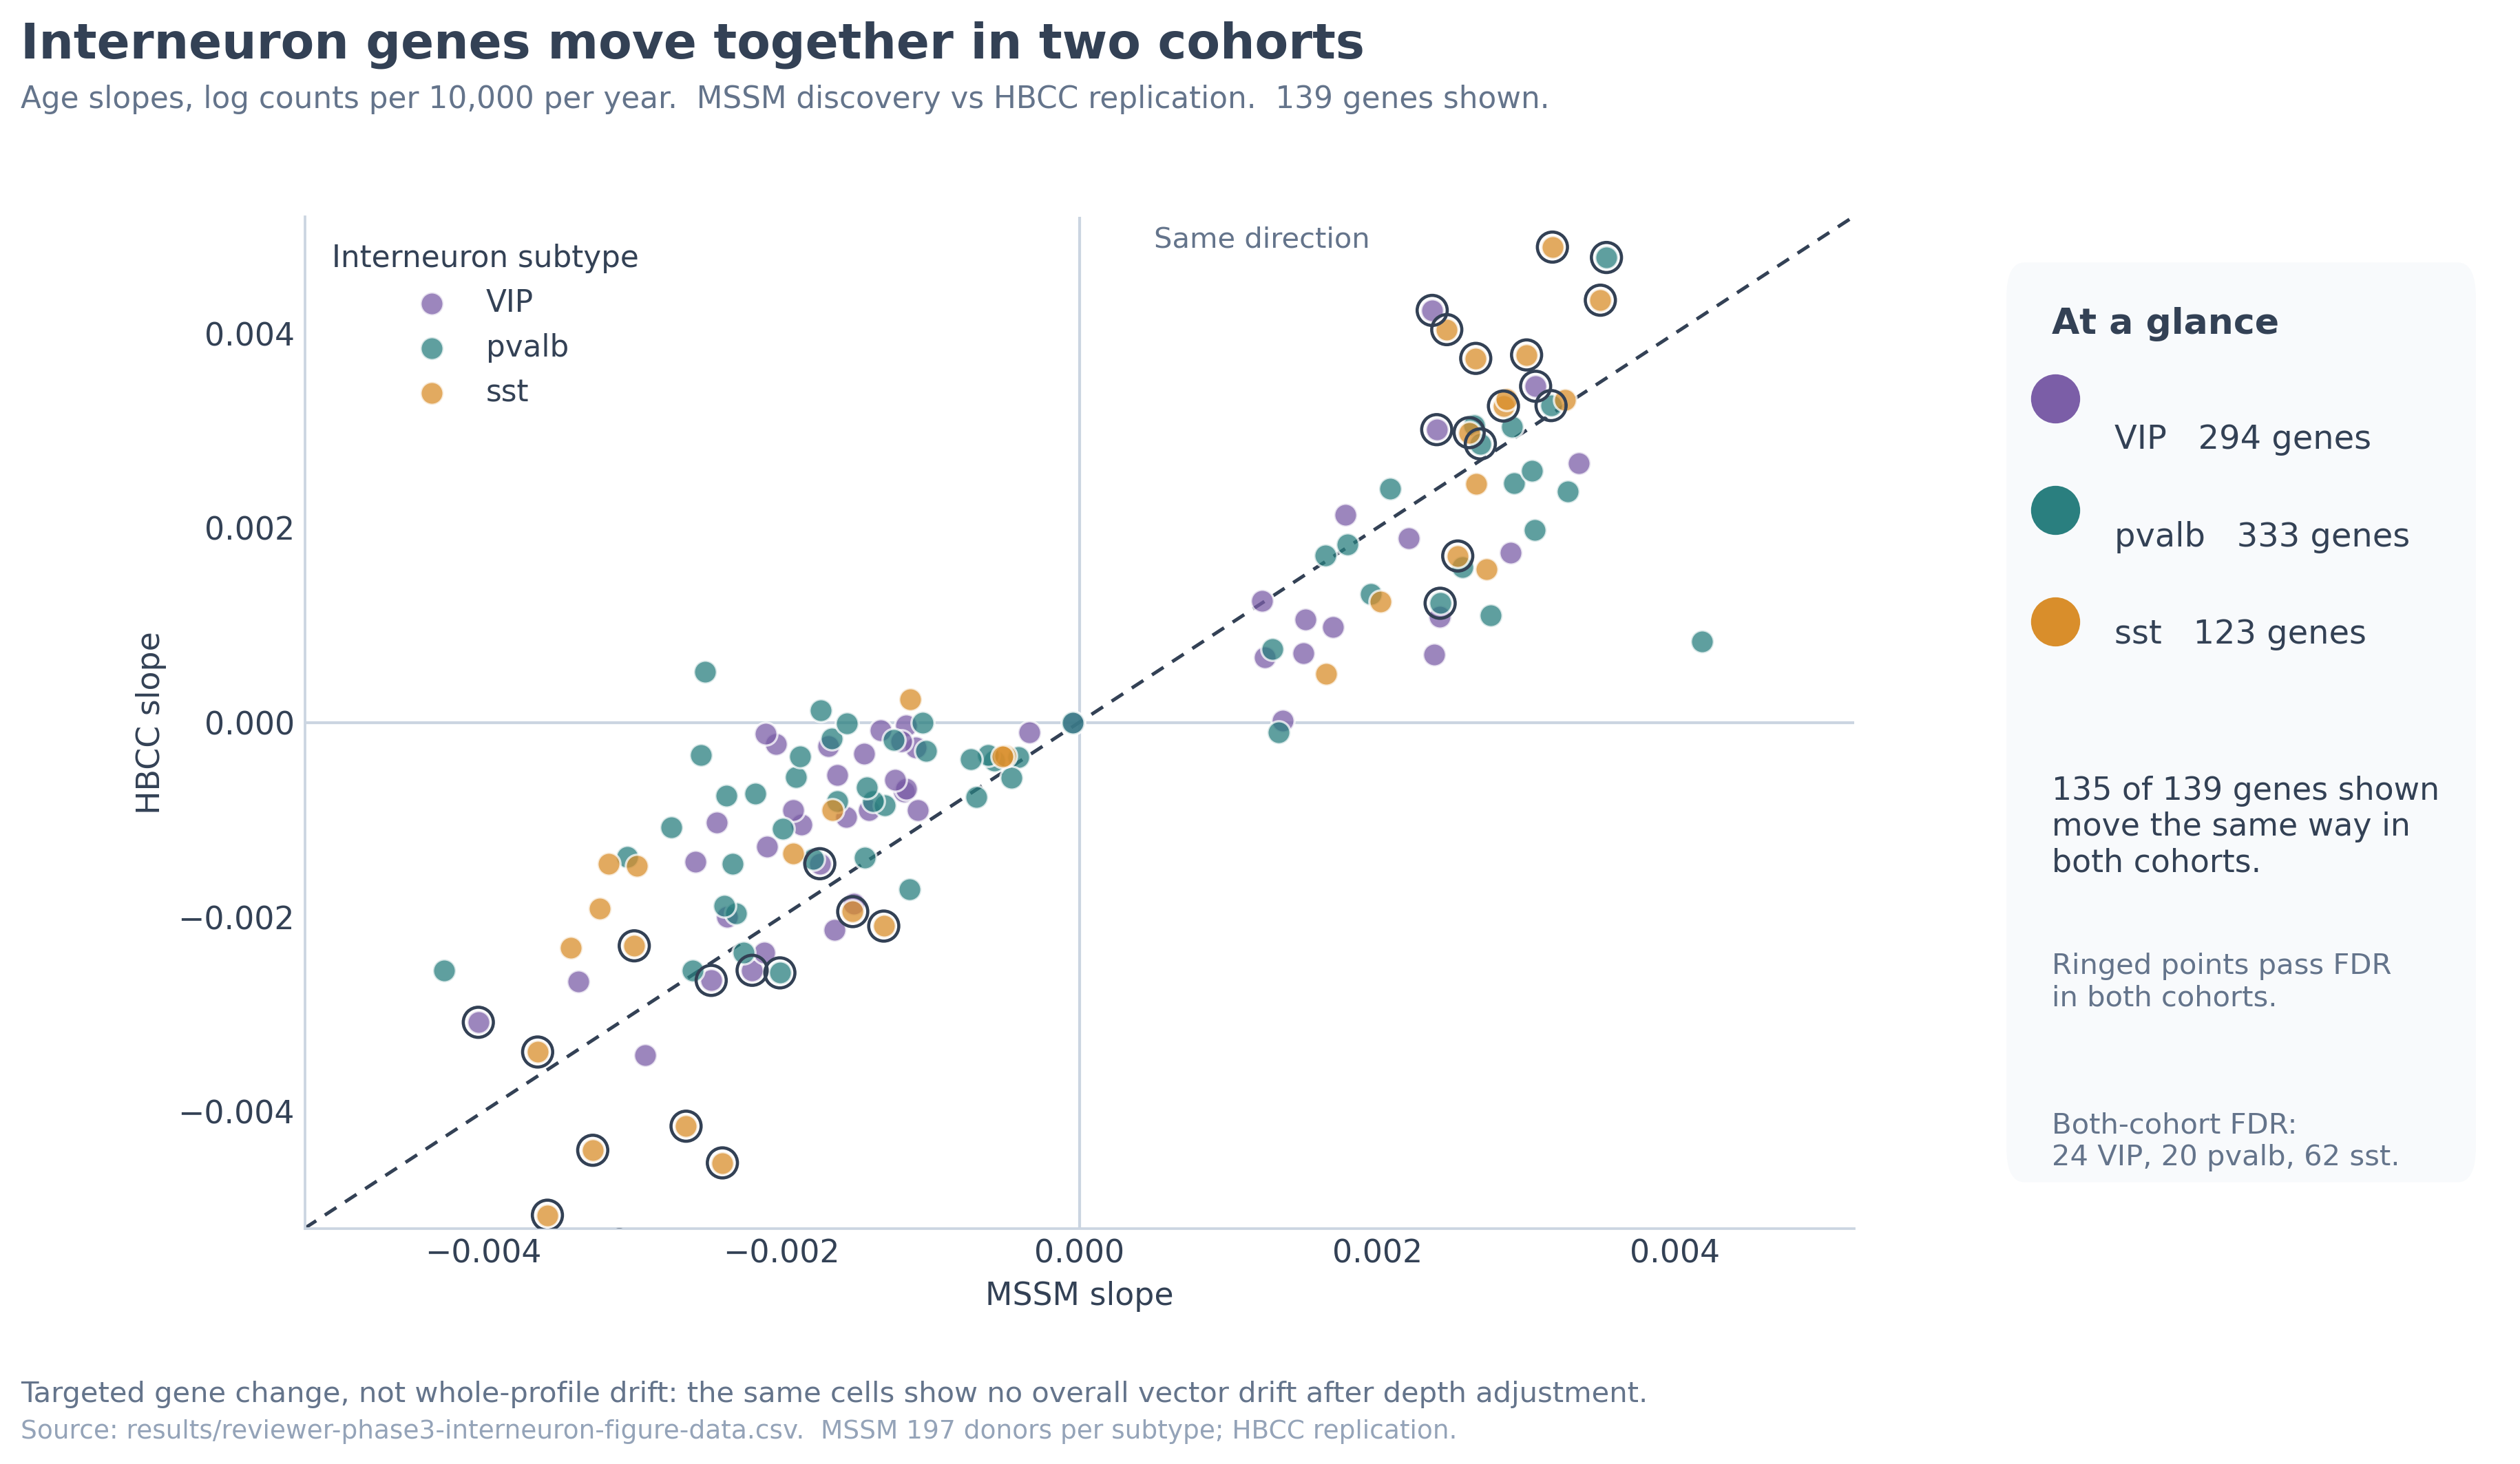
\includegraphics[width=0.92\textwidth,height=0.42\textheight,keepaspectratio]{figures-v2/fig4-interneuron.png}\caption{Figure 4. Interneuron gene changes. Each point is one gene in one interneuron subtype; the axes are its MSSM age slope and its HBCC age slope, in log counts per 10,000 per year, from depth adjusted donor pseudobulk models. 139 genes are shown; 135 move in the same direction in both cohorts. Ringed points pass false discovery rate in both cohorts. The side panel gives the full analysis totals (VIP 294, pvalb 333, sst 123 genes; both cohort false discovery rate 24, 20, 62). The figure does not prove causation, or establish that every displayed gene replicates at false discovery rate in HBCC. Data: results/reviewer-phase3-interneuron-figure-data.csv.}\end{figure}

\subsection*{A schematic summary}

Figure S1 states the argument of this paper as a schematic. Aging is defined operationally by the three measurements stated in the Introduction. Mouse shows distributed whole-profile drift, human shows targeted interneuron gene change without overall drift, and both show local fraction shifts. Any unitary theory must explain that pattern, and the decisive next experiment is a same-cell multiome with a causal perturbation and a rescue arm. Figure 5 presents the same argument with its two data panels.



\begin{figure}[htbp]\centering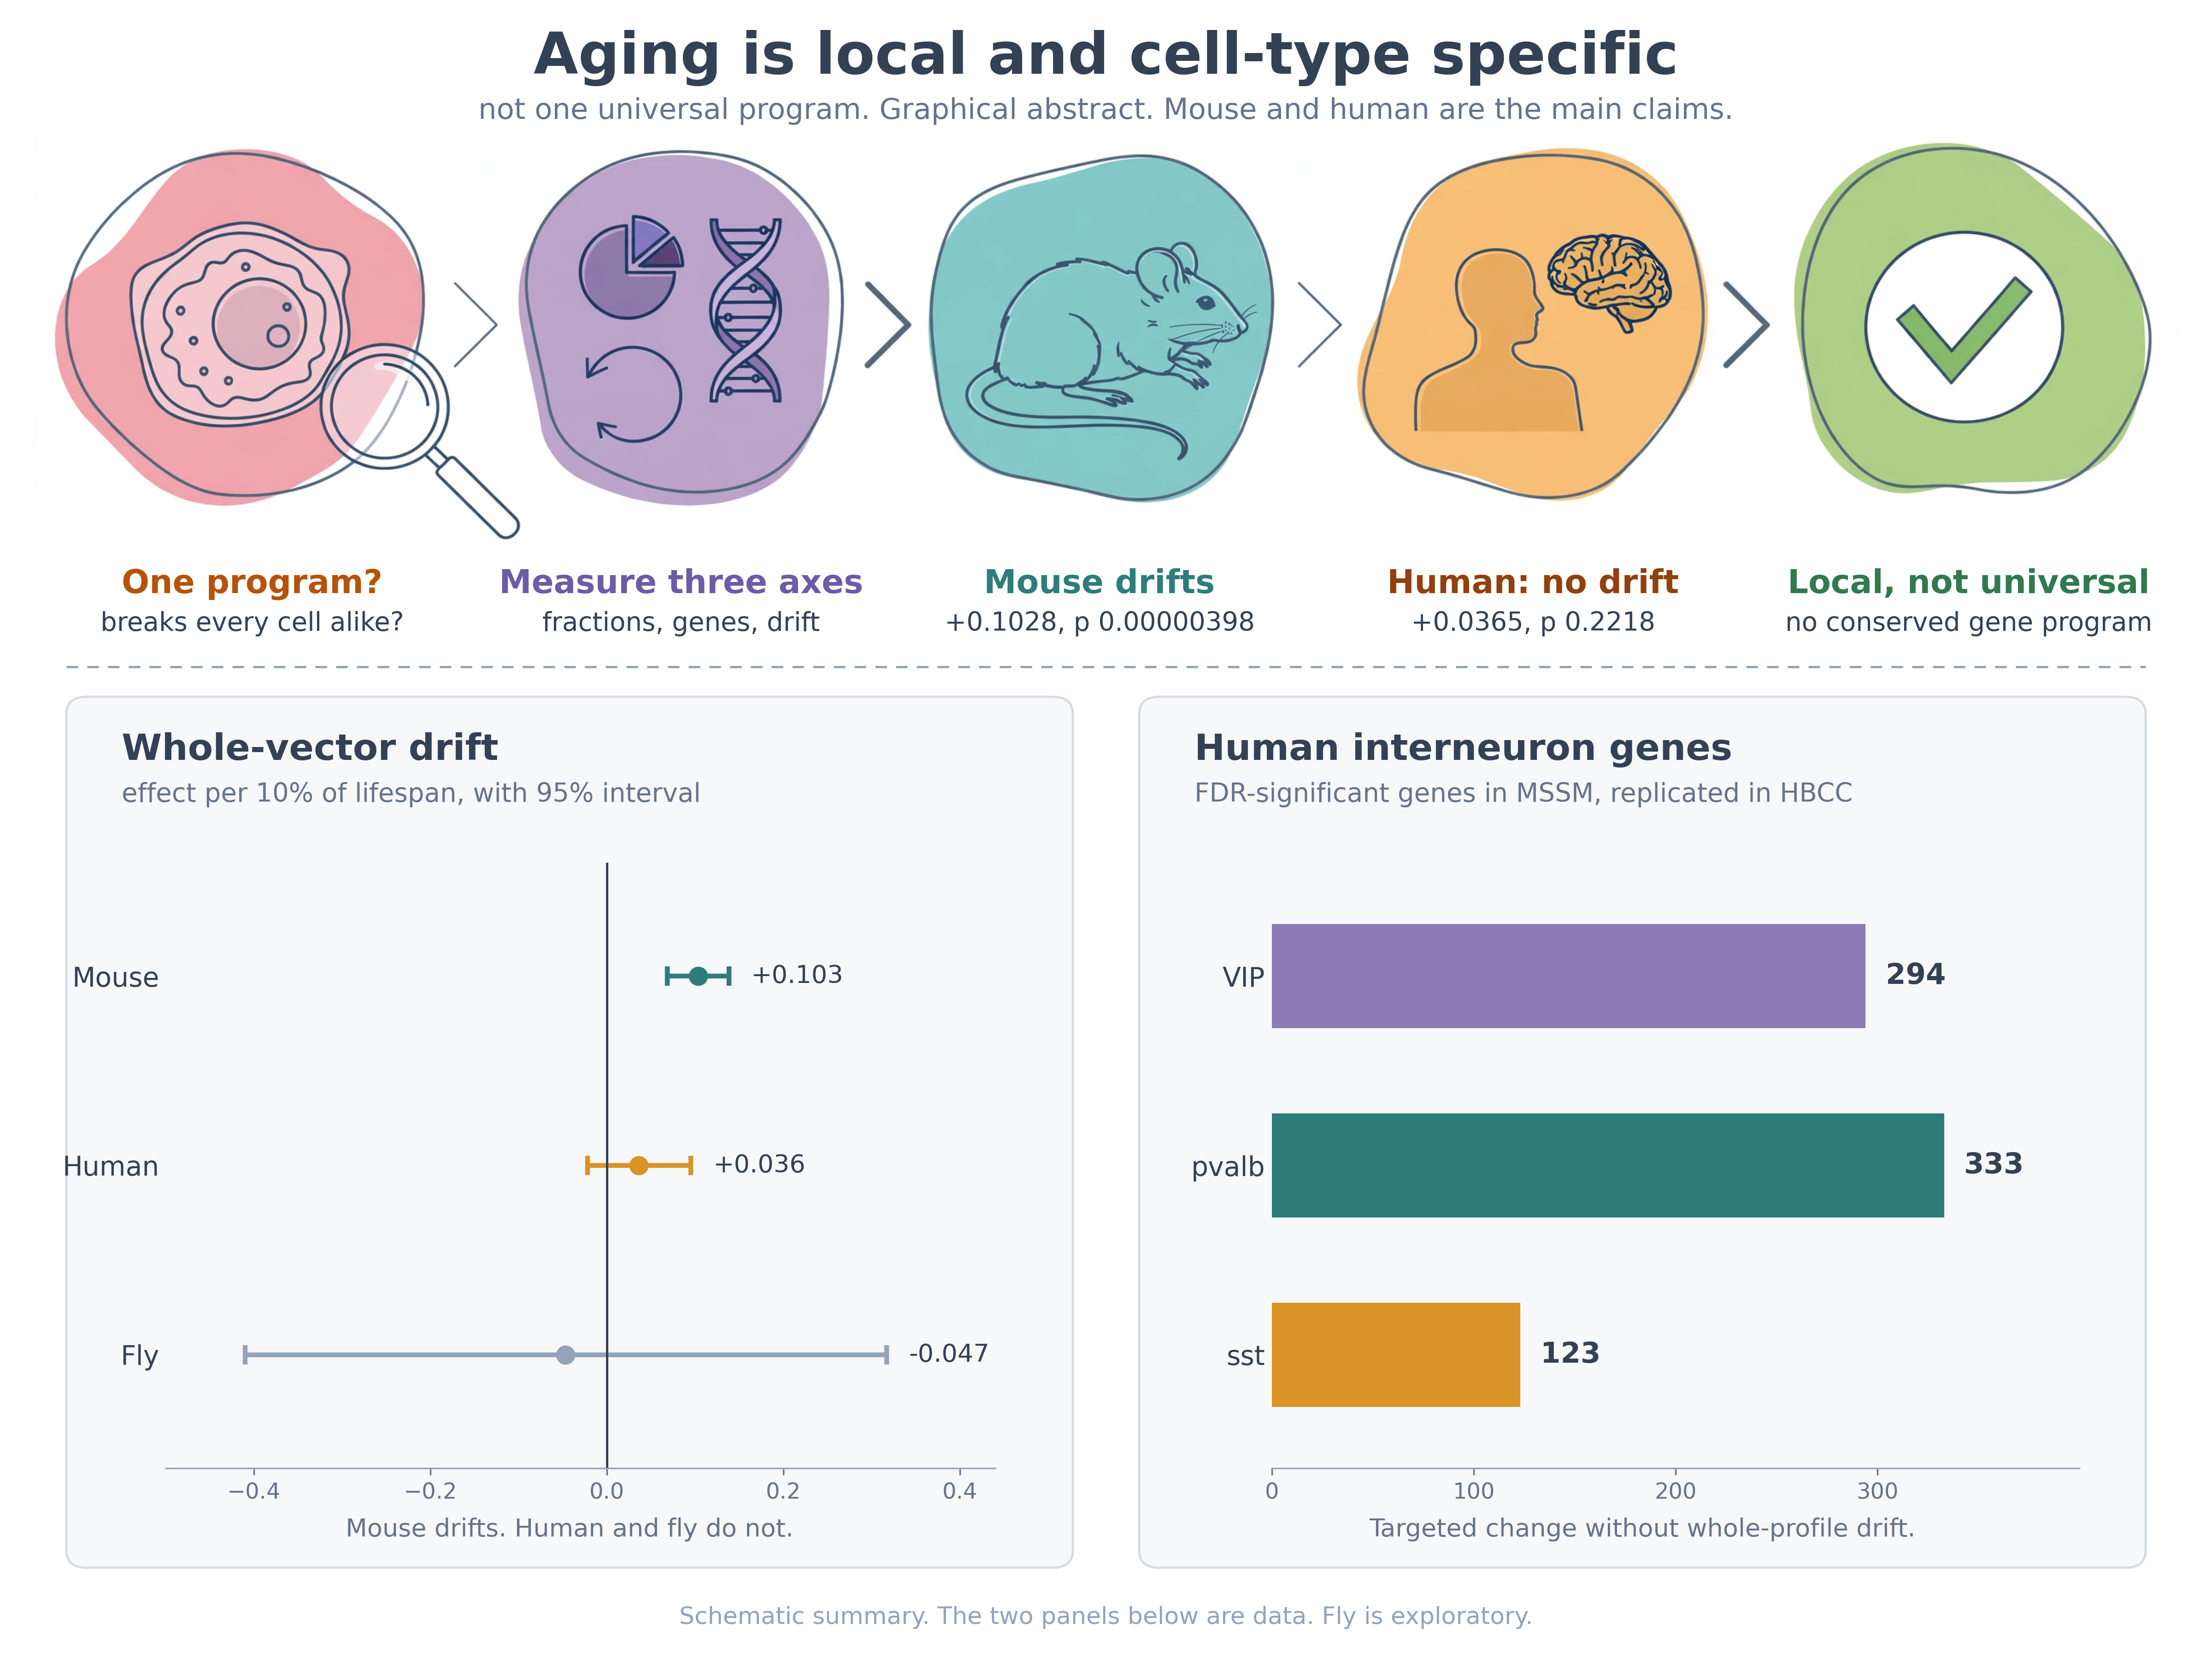
\includegraphics[width=0.92\textwidth,height=0.42\textheight,keepaspectratio]{figures-v3/fig6-final-mygen.png}\caption{Figure 5. Top row: illustration generated with Muse's own image generation from the style of published graphical abstracts, with labels added afterwards; the illustration itself contains no text or numbers. Bottom row: whole vector drift in mouse, human, and fly, and human interneuron gene counts. This is a summary schematic with two data panels; the numbers shown are the verified effects reported in the text.}\end{figure}



\subsection*{Off program expression does not increase at any depth, and the null stays imprecise}

The direct test of leaky, irrelevant gene transcription was run in mouse lung only. Off program expression is the fraction of transcripts from genes that are uncommon in young cells of the target type but characteristic of another lung cell type. The first draft measured this outcome only after downsampling every cell to 1,500 UMIs, which loses rare transcripts first. The reviewer response therefore ran a depth sweep at 500, 1,500, and 3,000 UMIs per cell and at full depth, with young reference marker definitions fixed across depths, plus a library size covariate arm at full depth. The 1,500 UMI point estimates reproduce the original global effects.


{\footnotesize\begin{longtable}{lllllll}

Depth & Off program effect per 15 months & 95 percent CI & p value & Entropy effect per 15 months & 95 percent CI & p value \\

\hline

500 UMIs & +0.2537 & -0.2237 to +0.7311 & 0.2751 & -0.0716 & -0.4992 to +0.3559 & 0.7260 \\

1,500 UMIs & +0.2438 & -0.2349 to +0.7225 & 0.2948 & -0.0789 & -0.5135 to +0.3557 & 0.7041 \\

3,000 UMIs & +0.1726 & -0.3506 to +0.6958 & 0.4928 & +0.0080 & -0.4144 to +0.4304 & 0.9683 \\

Full depth & +0.1743 & -0.3557 to +0.7044 & 0.4940 & -0.0906 & -0.5517 to +0.3704 & 0.6812 \\

Full depth, library size adjusted & +0.1590 & -0.3358 to +0.6539 & 0.5038 & -0.0602 & -0.3522 to +0.2318 & 0.6668 \\

\end{longtable}}

No depth produced a significant positive global off program association, so the prespecified withdrawal criterion was not met. The full depth null supports the previous null interpretation, but it does not prove biological stability: in the Phase 1 interval analysis the off program minimum detectable effect at 80 percent power was 0.6191 standard deviations, and equivalence was established at neither the 0.1 nor the 0.25 standard deviation margin. The entropy null is in the same position, with a minimum detectable effect of 0.5621 standard deviations and no equivalence at either margin.


A separate direct endpoint tells a different story about mouse lung, and the two must not be merged. The cell type average expression vector analysis, rerun without downsampling, gave an unadjusted Hellinger global effect of plus 0.2914 standard deviations per 15 months (95 percent confidence interval minus 0.1203 to plus 0.7030, p = 0.1653). After mean log UMI adjustment it was plus 0.2626 standard deviations (95 percent confidence interval plus 0.0806 to plus 0.4445, p = 0.00468). This endpoint measures displacement from young profiles. It is not off program expression and it is not entropy.


\subsection*{Adult only models, nonlinear age, and annotation stability}

Every public human vector and composition donor was already at least 20 years old. The minimum age across both analyses was 20, so adult only refitting uses the same donor sets and changes nothing for these public analyses. Developmental donors in PsychAD belong to the separate signature transport analysis. Nonlinear models used a fixed three degree of freedom cubic B spline. MSSM had two linear false discovery rate hits and no nonlinear hits in the vector analysis, and six linear hits and one nonlinear hit in the composition analysis. Integrated lung had two linear composition hits and no nonlinear hits. These results should not be summarized as confirmation of linear age effects, because nonlinearity and cohort specific age coverage can change individual conclusions.


Annotation stability limits how far the composition results can be pushed. No per cell annotation confidence probability was available in the mouse or public human inputs, and doublet scores were not relabeled as annotation confidence. Age related differences in excluded or unassigned cells were detected in integrated human lung (Spearman rho = +0.4334, q = 0.0251 across 48 ages) and in mouse pancreas (rho = +1.0 across four age groups, a result with only four groups that should not be generalized). A fixed canonical marker analysis found eight false discovery rate significant changes across 187 tests, seven in human and one in mouse, including increased microglial C1QA in MSSM (slope +0.00522 log counts per 10,000 per year, q = 0.000280) and decreased mouse cardiac fibroblast COL1A1 (slope -0.0397, q = 0.00617). These findings do not demonstrate identity loss, because marker expression can change without loss of cell identity. They do mean that identity loss cannot be excluded as an explanation for any affected composition result.


\subsection*{Exploratory and supplementary arms}

The following arms are exploratory or supplementary under the working scope of this revision. They are reported so that the record is complete, and none of them drives the main claims.


In fruit fly, gene effect concordance was plus 0.1936 against a null mean near zero, and the bidirectional vector hits were not independent at the gene level: among 703 pairs of the 38 depth adjusted vector hit cell types, 537 pairs shared at least one false discovery rate significant gene and 480 pairs had hypergeometric q below 0.05, with a median Jaccard index of 0.0130. Gene Ontology enrichment was concentrated in specific units rather than one common pathway across all hits. In worm, the vector result depends on the reference: plus 1.6755 standard deviations with a day 1 reference (permutation p = 0.00250), against plus 0.5319 with the balanced day 6 reference (parametric p = 0.0189, permutation p = 0.0535). Day 6 is the primary reviewer response reference because it includes both sequencing platforms. In zebrafish, the fine grained vector effect was plus 0.2211 with a wide interval (95 percent confidence interval minus 0.3588 to plus 0.8009) and no equivalence at either stated margin, in six fish for the fine grained analyses. In naked mole rat, the vector point estimate was minus 0.4744 (exact p = 0.2) in five animals with skin only data, and the concordance analysis was unresolved because the permutation null itself was already high (observed +0.6146 against a null mean of +0.6423, p = 0.7000). Neither arm supports a verdict on stability or on a difference from other species.


The proliferation moderator analysis is post hoc and classifies annotated identity rather than measuring turnover. Its absolute contrasts were minus 0.0033 standard deviations for cell fractions and minus 0.0051 standard deviations for expression vectors. In the interval analysis, the fraction contrast established equivalence at the 0.1 standard deviation margin, and the expression contrast established equivalence only at the 0.25 standard deviation margin. The arms are uneven, with only two post mitotic mouse expression units and only one proliferative worm unit, and naked mole rat was excluded.


The methylation clock analysis is a benchmark reproduction, not validation. Applying the published Universal Clock 2 coefficients without refitting gave a predictive R squared of 0.6383 in the human multi tissue evaluation, with a mean absolute error of 5.06 years across 661 human profiles, and a predictive R squared of 0.3169 in mouse liver, with a mean absolute error of 0.36 years, scored with 724 of 816 clock probes. GSE184211 is confirmed to be part of the consortium resource used to develop the published clocks. For GSE199979, the publisher supplementary workbook was checked, 93 sheets checked, and contained no occurrence of the accession, a tested sample identifier, or a tested sample title, so sample level membership in clock development remains unresolved. Unresolved is not evidence of no overlap.


\section*{Discussion}

The central result is a constraint. At the transcriptomic level, aging in mouse and human is cell type specific: composition changes in specific cell types in specific organs, gene changes concentrated in specific cell types, an overall expression displacement that is robust and distributed in mouse and small overall in human, and no consistent increase in off program expression at any measured depth. A strong universal program, in which one pattern of breakdown is imposed on every cell type, is not supported at the transcriptomic level. The concordance result adds the needed nuance: gene level age effects do share direction across cell types, so the local pattern is coordinated, not random. Coordination of direction is not a universal program of deterioration, and this paper does not claim that it is.


That constraint bears directly on single mechanism theories, including the proposal that DNA damage, followed by repair that scrambles epigenetic information, drives downstream inflammation, fibrosis, and transposon derepression. This paper neither proves nor disproves that proposal, and the reason is simple: its upstream steps were not measured here. Chromatin was not measured. DNA damage was not measured. Transposon RNA was not quantified. Protein and cell function were not measured. Actual turnover was not measured. What was measured is the downstream transcriptomic pattern such a theory would have to produce, and that pattern is local rather than universal. Fibrosis, in particular, is not demonstrated by any result here: fraction changes are changes in shares of recovered cells, not measurements of extracellular matrix deposition or of tissue takeover.


A middle position remains fully compatible with the data: a common maintenance vulnerability, shared across cells in how genome, epigenome, proteome, and energy are maintained over time, with divergent local manifestation that depends on each cell type and its chromatin landscape, repair capacity, division behaviour, niche, and exposure. On that view, a clock can track age across mammals, as the benchmark here reproduces, while the consequences of age in any given cell type stay local. Tracking time is not the same as causing dysfunction, and a shared vulnerability is not the same as one universal transcriptional program.


\subsection*{What the results do and do not say about existing theories}

The Information Theory of Aging, in its universal identity-loss form, is weakened by these results. It predicts that aging should erode cell identity everywhere, with leaky transcription and movement away from the young state in every cell type. The mouse data fit that prediction in broad outline, but the human data do not: human profiles show no overall displacement, and the strongest human change is targeted gene change in interneurons without global drift. The off-program test, the most direct transcriptomic test of leaky transcription in this study, found no increase at any depth, but its interval is wide, so it is inconclusive rather than a refutation. The chromatin version of the theory was never directly tested here, because this study measured no chromatin, DNA damage, transposon RNA, protein, or function in the same cells. A theory that lives upstream of the transcriptome cannot be settled by transcriptomic data alone.

The Hallmarks of Aging list is compatible with these results, but it is unpredictive as a list. Almost any local result can be assigned to one of its hallmarks after the fact, so the list predicts almost nothing specific in advance about which cell types should change, in which direction, or by how much. As a coordinated program, in which the hallmarks move together in every cell type, it is weakened by the same pattern that weakens a universal program: the changes are local, coordinated in direction at the gene level, and uneven across species.

Telomere and replicative senescence theories are weakened more cleanly. They predict that division history should organize the pattern of change, yet the proliferation contrast in this study is near zero, and the strongest human change is in post-mitotic interneurons, cells that do not divide. Division is therefore not the master clock of the transcriptomic pattern reported here.

Evolutionary theories that predict heterogeneity are supported in their plural prediction. Antagonistic pleiotropy, disposable soma, and mutation accumulation all predict that aging should appear as different failures in different cell types and species, under a common weakening of selection with age, rather than as one conserved program. That is the pattern these data show. Programmed aging, by contrast, is weakened: a program should leave a shared, directional signature, and no shared signature survives the tests in this study.

Two nulls in this paper must not be confused. The human overall vector null is evidence of absence: its interval sits inside a 0.1 standard deviation equivalence region (p = 0.0169), so a large overall human displacement is excluded at that margin. The mouse lung off-program null is absence of evidence: at full depth it is plus 0.1743 per 15 months, with a 95 percent confidence interval from minus 0.3557 to plus 0.7044 (p = 0.4940), a wide interval in which equivalence was not established. This paper does not claim that pluralism is proven as a metaphysical fact. It claims only that the transcriptomic data constrain any unitary theory: whatever single upstream process exists, its transcriptomic consequences are local, cell type specific, and species dependent, and any unitary theory must explain that pattern rather than assume it away.

The decisive future tests, in order, are: first, same cell measurement of chromatin, RNA, and a damage marker in the cell types that do and do not change; second, a causal damage or repair perturbation that tests direction rather than association; third, a rescue test, in which reversing the proposed upstream step should reverse the local pattern if the theory is right; fourth, direct transposon quantification rather than inference from gene level measures; fifth, a direct turnover test using Ki-67 or EdU labelling or lineage tracing, rather than annotated identity; and sixth, a preregistered universality prediction, stating in advance which cell types in a new cohort should change, in which direction, if a universal program exists.


For measurement practice, the results argue for cell type resolved designs as the default, with depth modelled in every distance or detection analysis, with composition and within cell expression reported as separate findings, and with multiplicity handled across the full family of tests actually run. The concrete starting points offered here for directed validation are the replicated interneuron gene changes first, on evidential strength, and the corrected signature associations second, with the PsychAD matched null caveat attached to the latter.


\subsection*{Limitations}

These limitations are part of the results, not qualifications added after them.


The study is cross sectional and observational throughout. There is no perturbation, no longitudinal follow up, and no causal identification. Age associations can reflect cohort composition, technical variation, development, disease, or postmortem effects.


Non significance is treated as absence only where an equivalence test at a stated margin supports it. The human overall vector null and the proliferation fraction contrast meet that standard at the narrow margin used here. The off program, entropy, naked mole rat, and zebrafish nulls do not, and they are reported as imprecise rather than as evidence of stability.


Fly and worm samples are pools, not individually tracked animals, so within pool variation is not available to the inference. The naked mole rat arm has five animals, with skin only and group level ages, and the zebrafish fine grained arm is small. Neither can support claims of stability, protection, or species difference.


PsychAD and the public MSSM and HBCC cohorts contain exact identifier confirmed overlapping donors, so PsychAD analyses are not independent replication of the public cohorts. The MSSM to HBCC interneuron comparison uses different source banks.


Annotation is fixed while marker expression changes with age, and excluded cell fractions differ by age in at least two datasets. Identity loss therefore cannot be excluded as an explanation for any affected composition result.


Clock training membership is unresolved for GSE199979 and at mouse sample level, so the clock results are a benchmark reproduction and cannot be presented as independent validation.


Depth, sequencing platform, and reference choice affect the measurements throughout. Platform and age are partly entangled in worm, and the worm vector effect changes size and security with the reference age.


Cross species effect sizes are standardized within each dataset. They are not directly comparable as measures of biological importance, because tissues, age windows, assays, annotation resolution, and lifespan coverage differ between species.


\section*{Conclusions}

Together, these results rule out a single universal transcriptional program of aging at the level measured here. Fractions shift only in specific cell types in specific organs, whole expression profiles drift in mouse but show no overall drift in human, off program expression does not increase at any measured depth, and the durable human finding is targeted gene change in interneurons across two cohorts. Gene level effects share direction across cell types more than chance allows, which shows coordination without a universal breakdown. Any shared upstream process must therefore have consequences that differ by cell type, and any unitary theory of aging must explain that pattern rather than assume it away. The decisive next step is a same-cell multiome measurement with a causal perturbation and a rescue arm.


\section*{Data Availability}

The analysis code and committed aggregate result tables are in the Agescape repository. Dataset accessions are given in the Materials and Methods. The results published here are in whole or in part based on data obtained from the AD Knowledge Portal (NIH-NIA, U24AG061340). Controlled access PsychAD donor level values (Synapse syn52396927, pseudobulk resource syn62064518) are available from the source resource under its own terms and were not redistributed; only aggregate results are shared here.


\section*{Funding}

The author received no external funding for this work. [Pending author confirmation.]

\section*{Competing Interests}

The author declares no conflict of interest. [Pending author confirmation.]

\section*{Ethics Statement}

This study performed no new human or animal work. All data analyzed are from published public cohorts and controlled access resources used under their own terms, as described in the Materials and Methods. No new human participants or animals were recruited, no interventions were performed, and no identifiable individual level data are reported. [Draft statement, pending author confirmation. No ethics approval number is claimed.]


\section*{Acknowledgements}

The author thanks the peer reviewers whose reports prompted the Phase 1 to 3 reanalyses reported here.


\section*{Supporting Information}

The following figures support the main text and are not main figures. Figure S1 is the schematic summary of the argument, Figure S2 is the story diagram, and Figure S3 is the evidence map.

\begin{figure}[htbp]\centering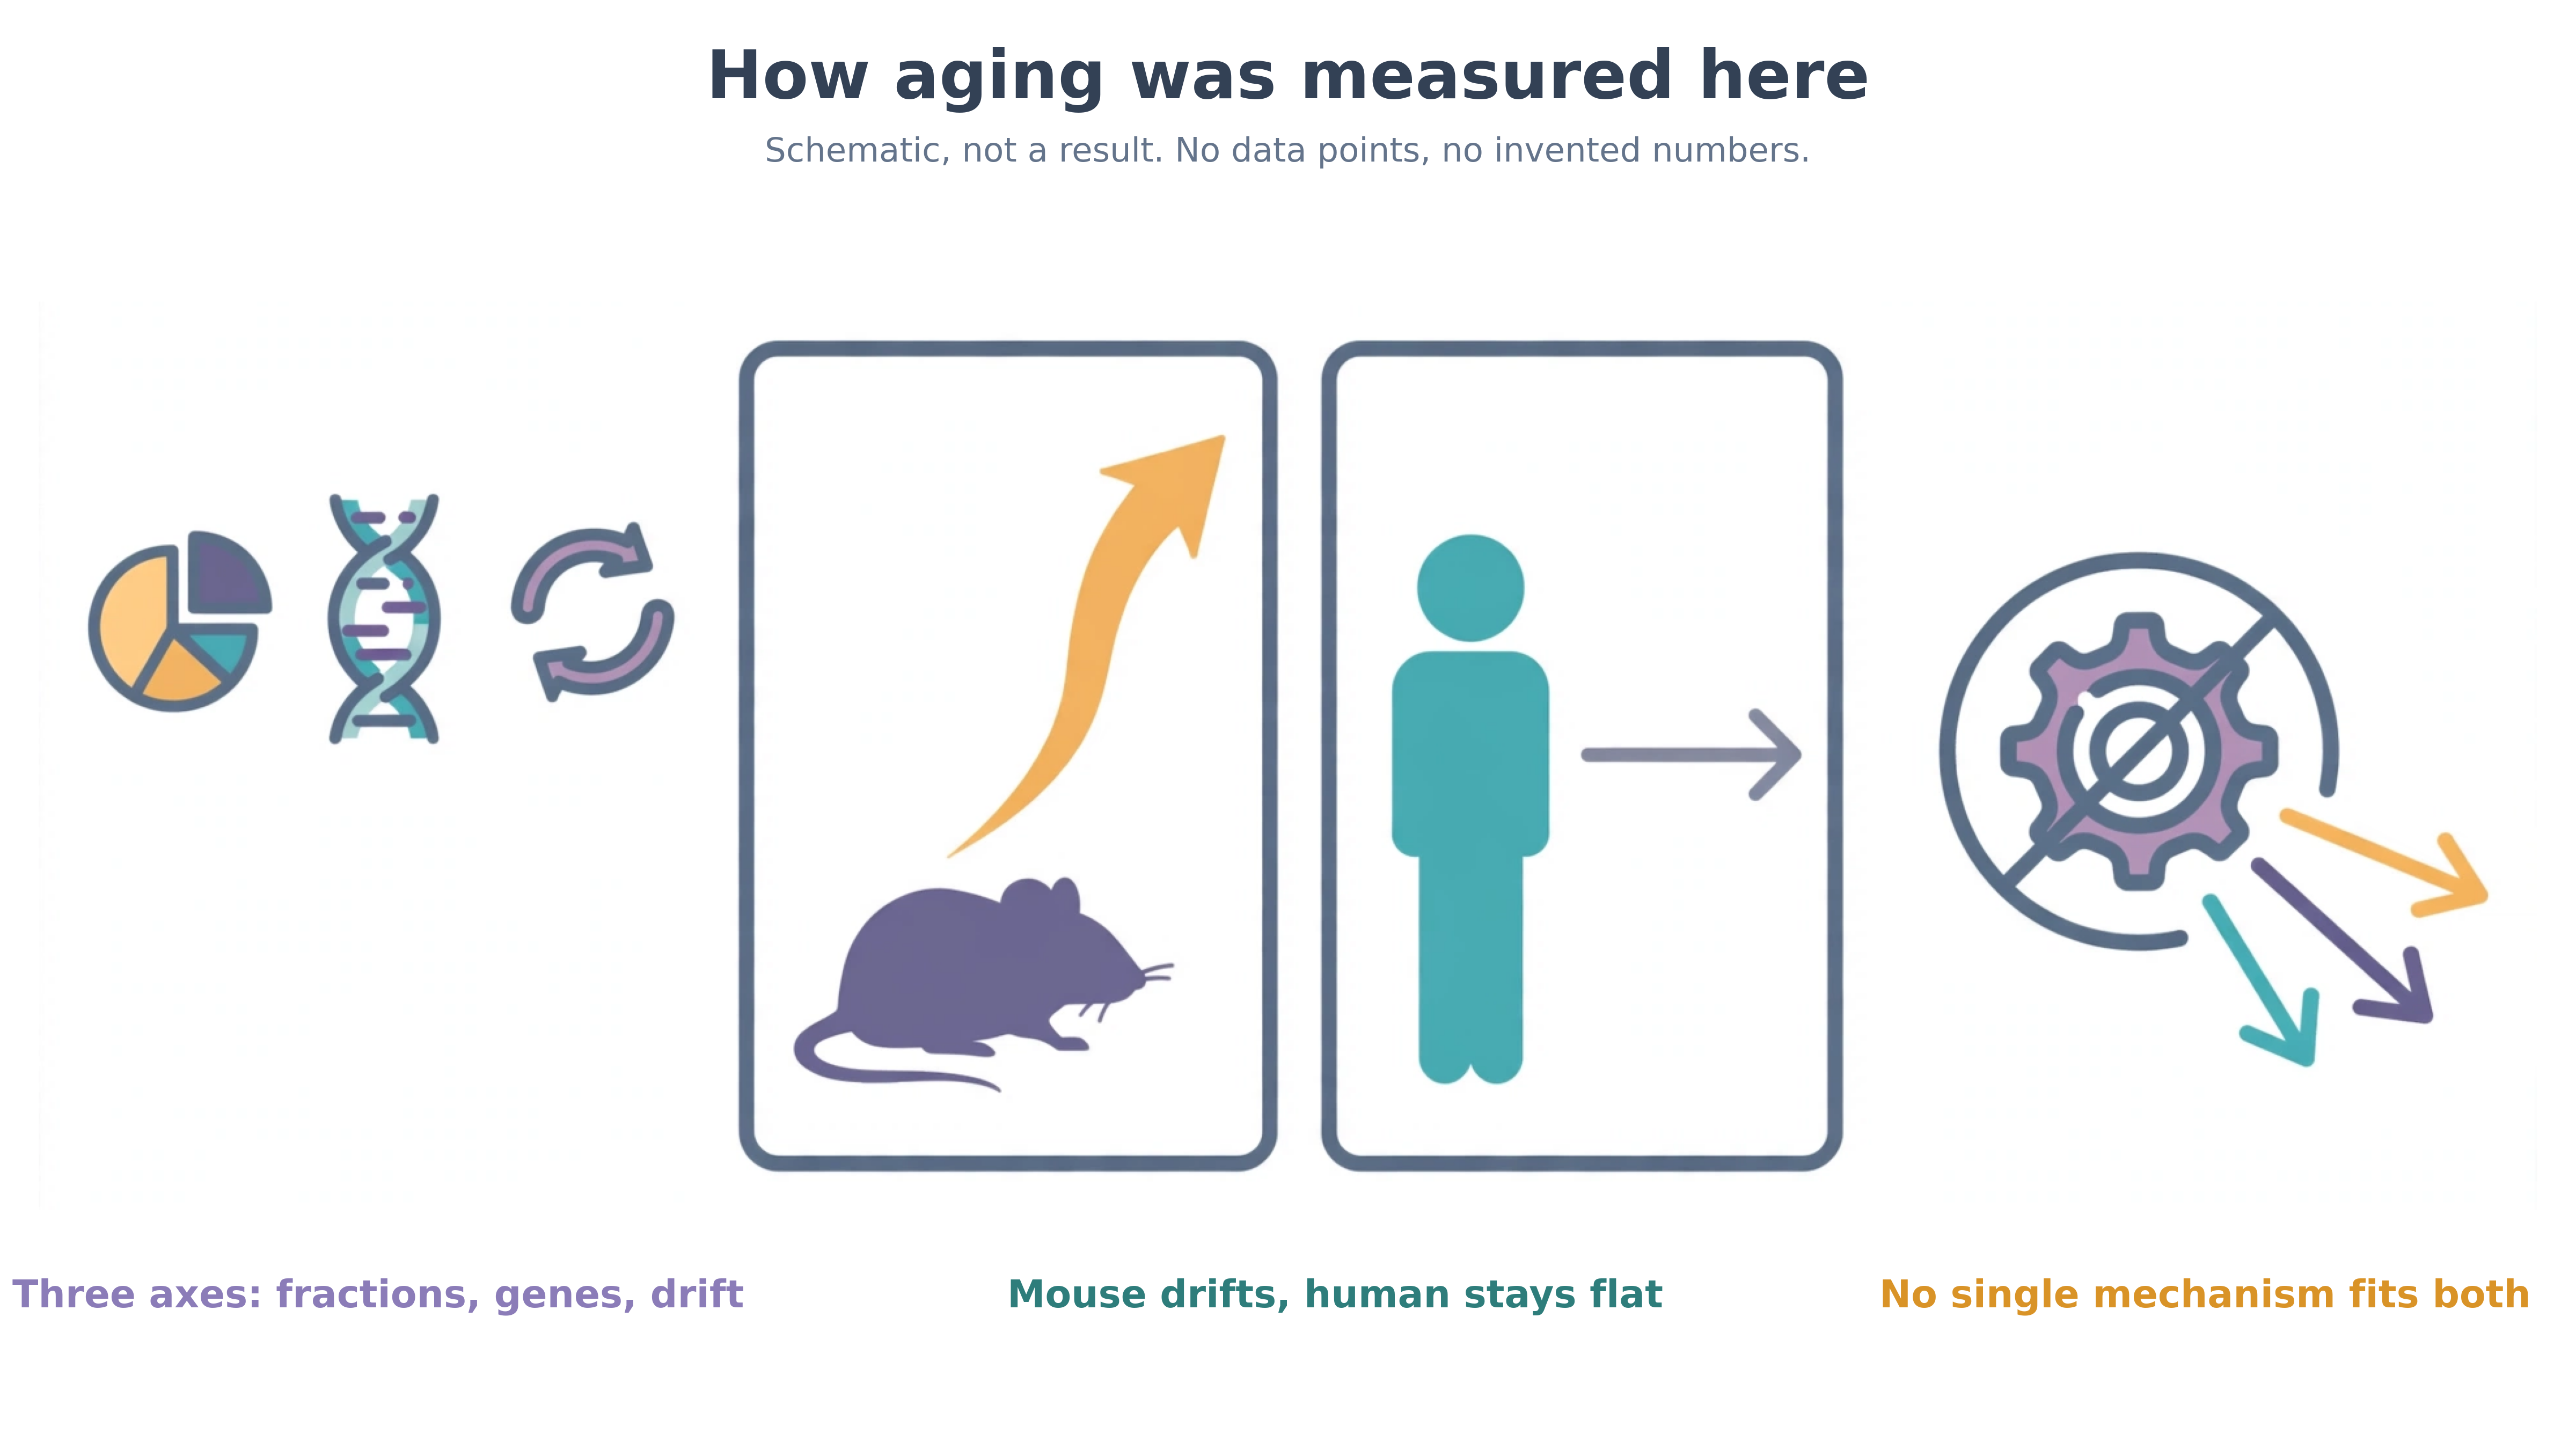
\includegraphics[width=0.92\textwidth,height=0.42\textheight,keepaspectratio]{figures-v3/fig5-final-mygen.png}\caption{Figure S1. Schematic summary of the operational definition, the mouse versus human pattern, and the constraint on unitary theories. The art was generated with Muse's own image generation from the style of published graphical abstracts, with labels added afterwards; the art itself contains no text or numbers. This is a schematic, not a result. It contains no data points, no invented numbers, and no error bars.}\end{figure}

\begin{figure}[htbp]\centering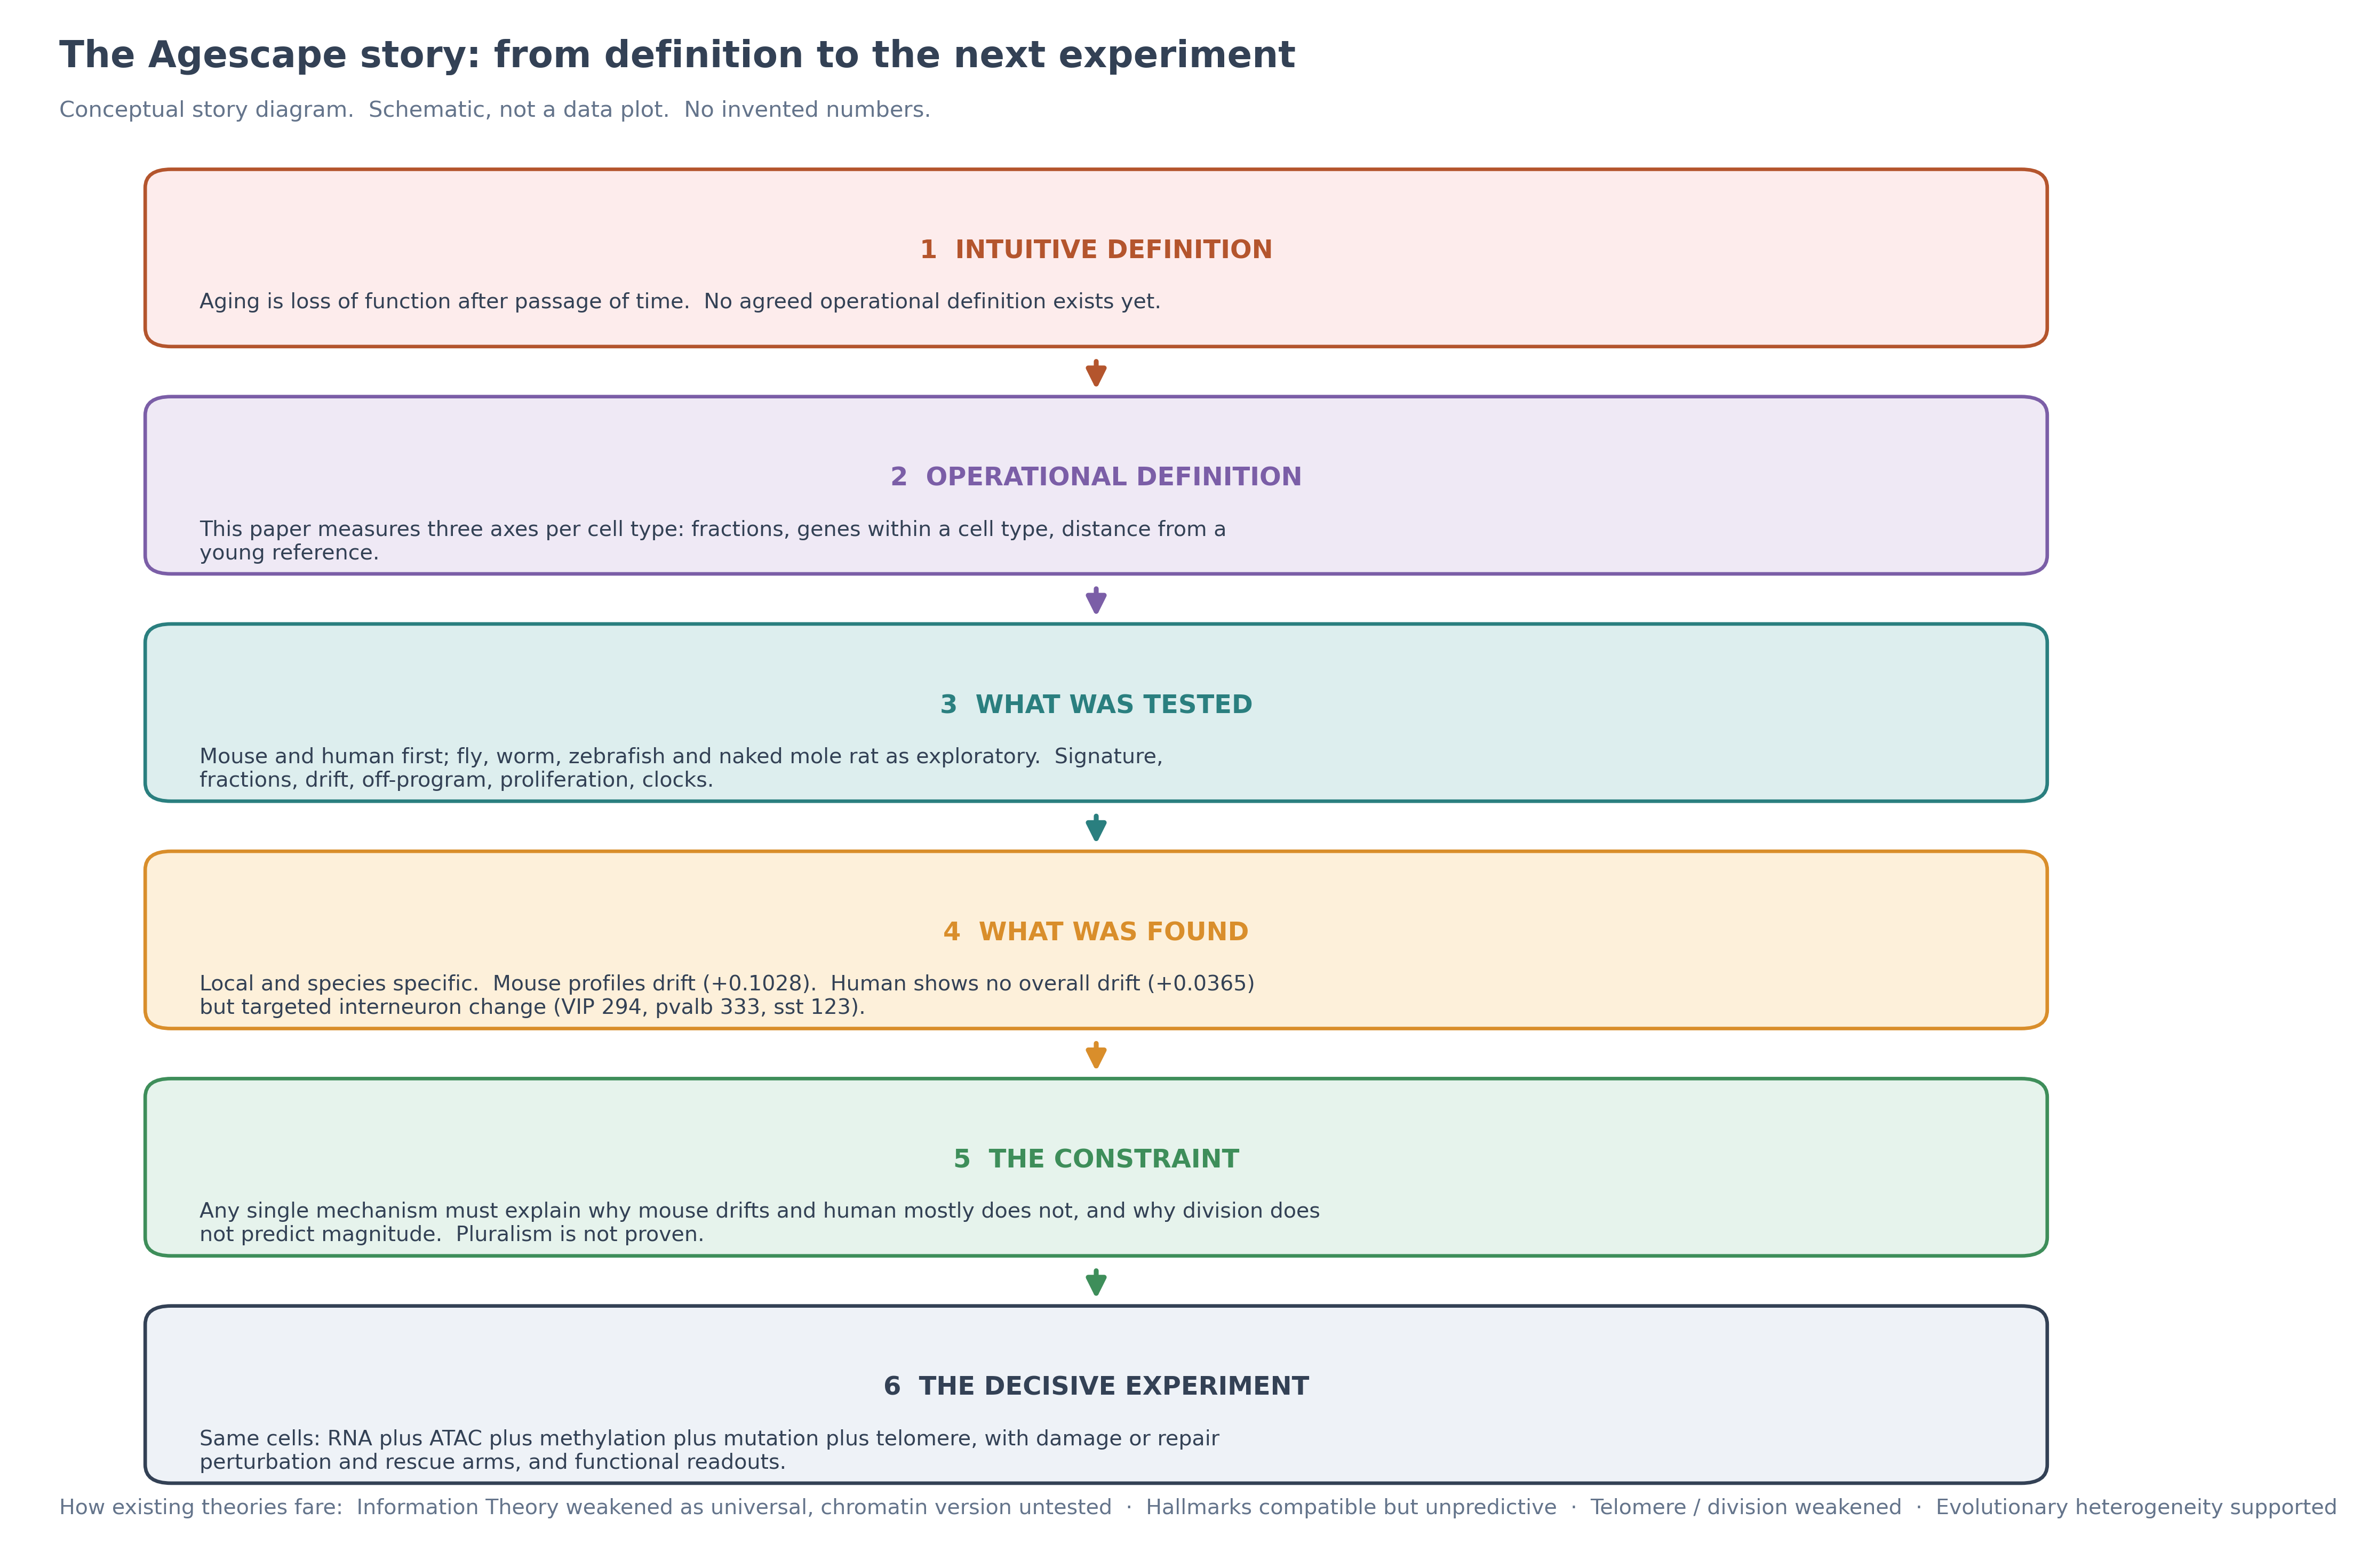
\includegraphics[width=0.92\textwidth,height=0.42\textheight,keepaspectratio]{figures-v2/fig7-story-diagram.png}\caption{Figure S2. Story diagram. From the intuitive definition of aging, through the operational definition used here, what was tested, what was found, the constraint on unitary theories, and the decisive next experiment. This is a schematic, not a result. The decisive experiment is proposed, not done here.}\end{figure}

\begin{figure}[htbp]\centering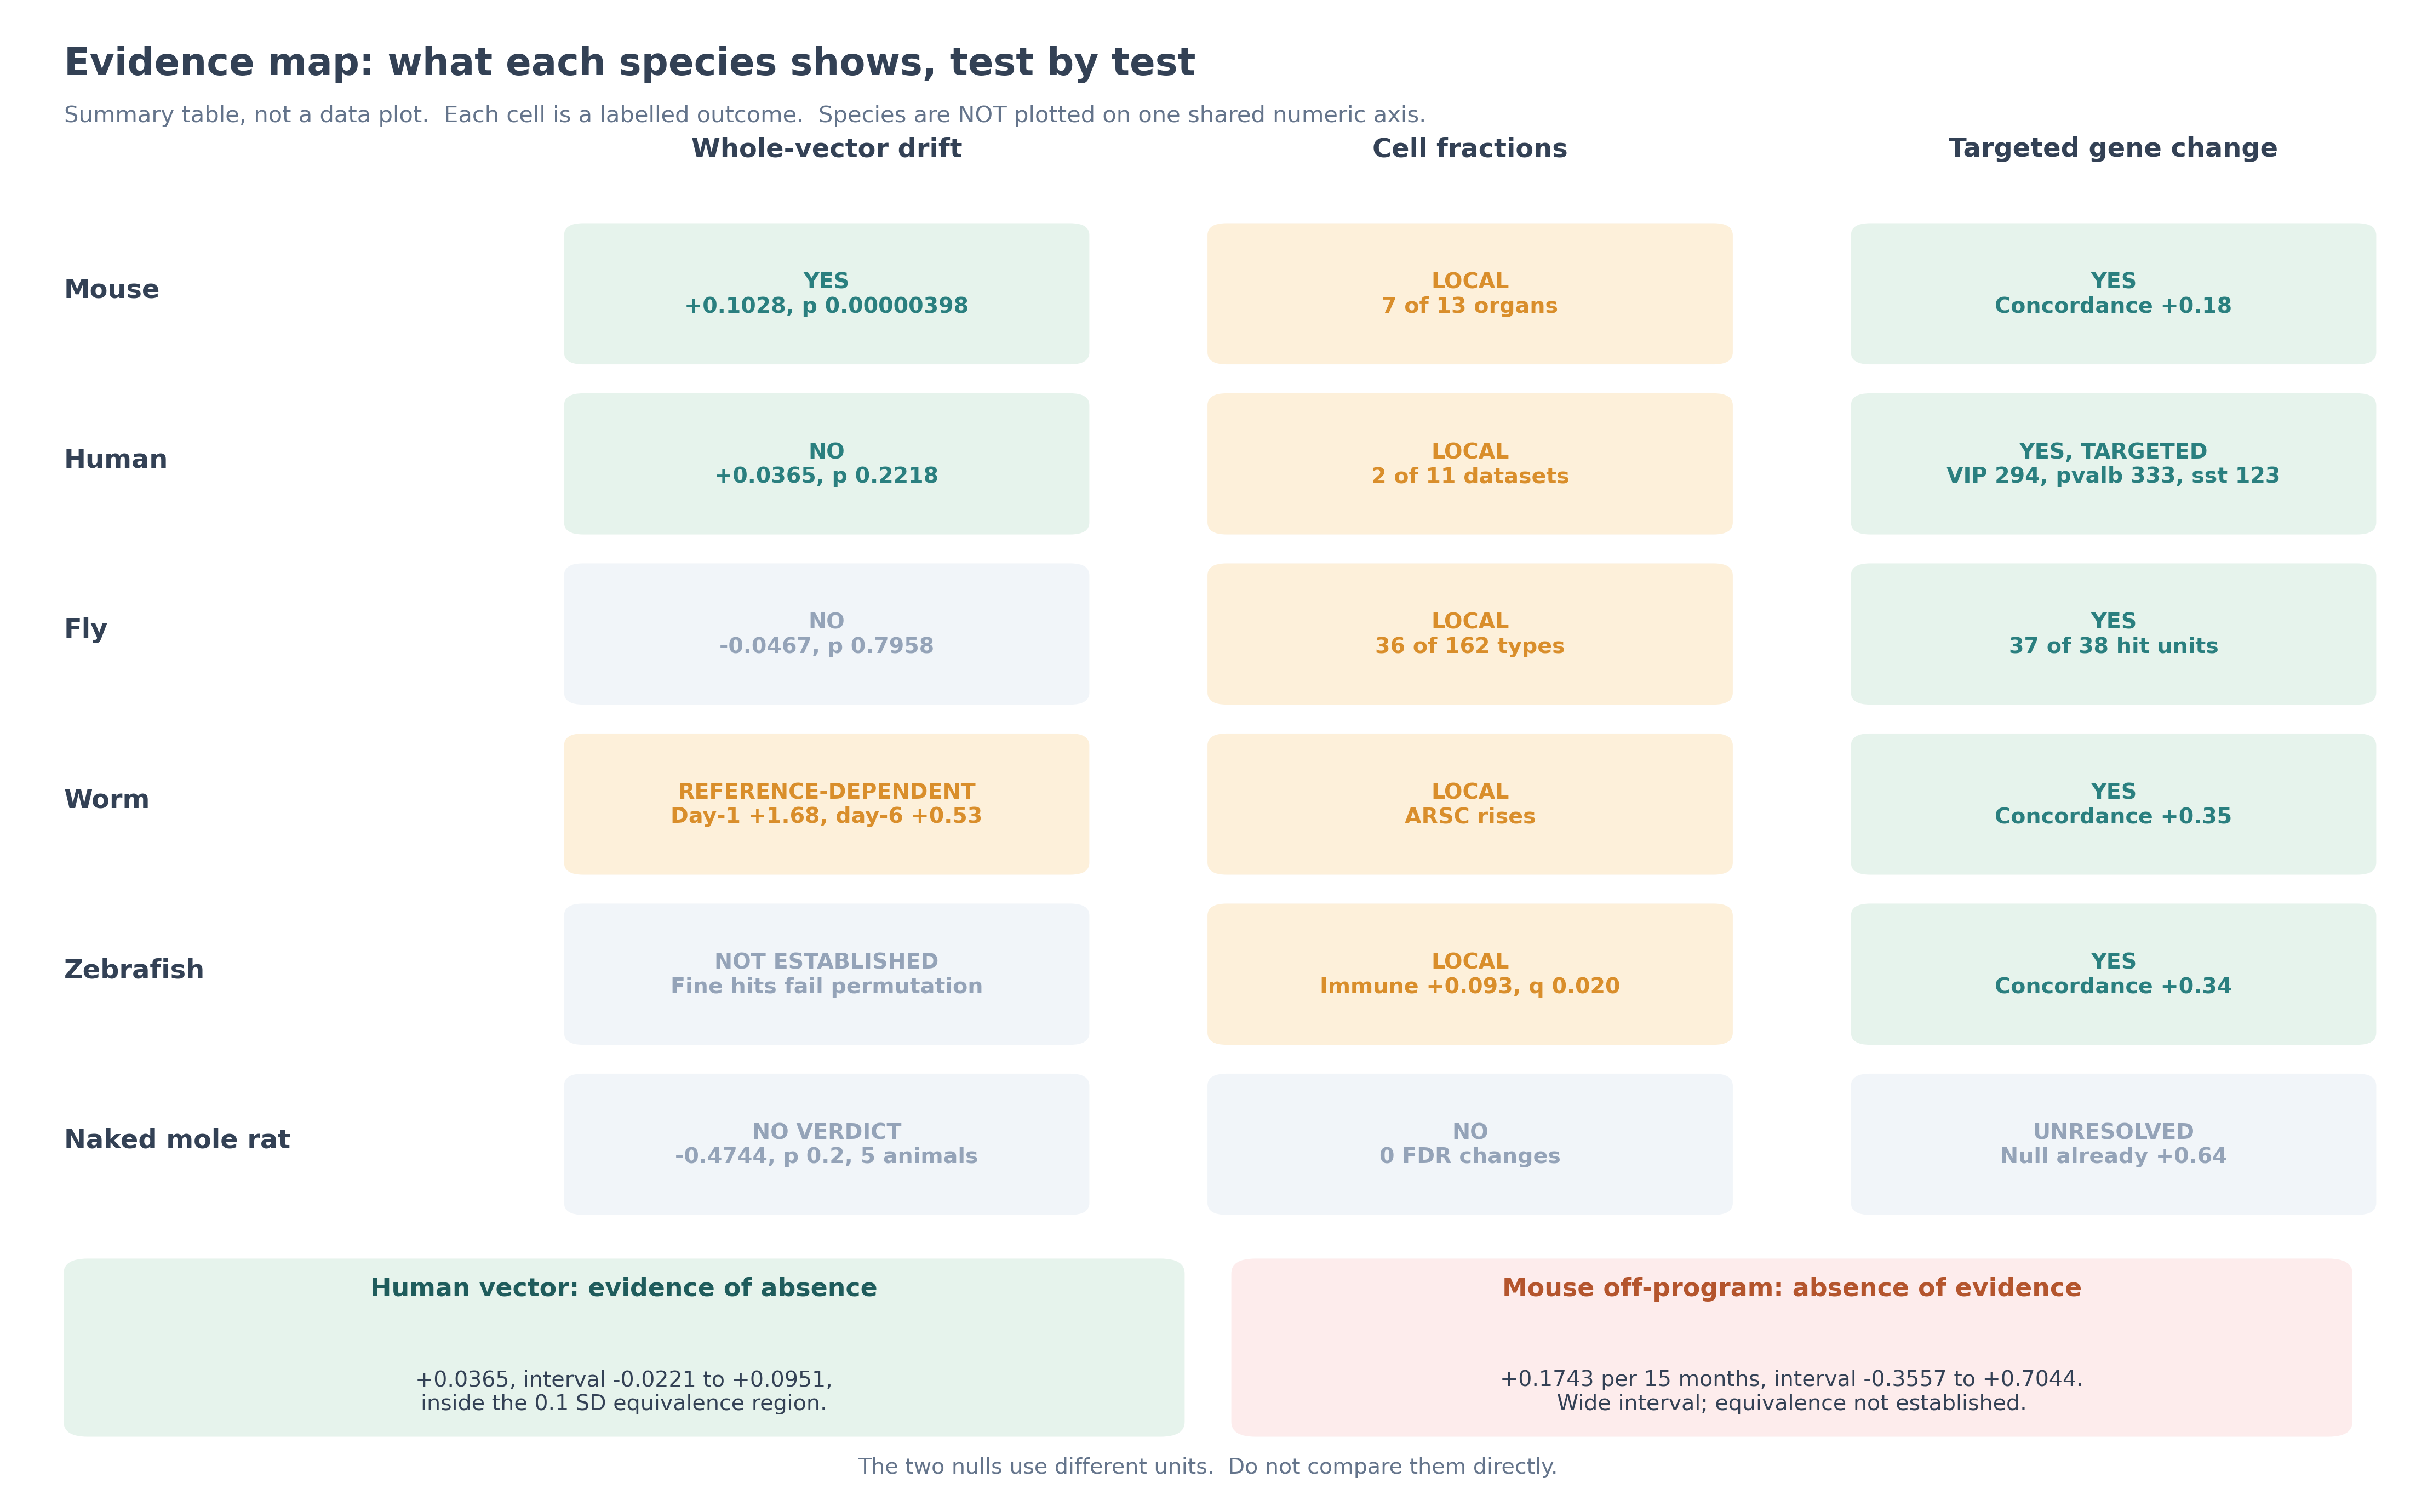
\includegraphics[width=0.92\textwidth,height=0.42\textheight,keepaspectratio]{figures-v2/fig8-evidence-map.png}\caption{Figure S3. Evidence map. What each species shows for whole vector drift, cell fractions, and targeted gene change. The bottom panels separate the two Bayesian nulls: the human vector null is evidence of absence, the mouse off-program null is absence of evidence, and the two use different units. This is a summary table, not a data plot.}\end{figure}

\section*{References}

References 1 to 32 were verified against Crossref metadata in the Phase 3 audit, with title similarity of at least 0.85. Author lists are abbreviated as in that audit.


1. Almanzar N, Antony J, Baghel AS, Bakerman I, Bansal I, et al. (2020). A single-cell transcriptomic atlas characterizes ageing tissues in the mouse. Nature. https://doi.org/10.1038/s41586-020-2496-1


2. The Tabula Sapiens Consortium, Jones RC, Karkanias J, Krasnow MA, Pisco AO, Quake SR, et al. (2022). The Tabula Sapiens: A multiple-organ, single-cell transcriptomic atlas of humans. Science. https://doi.org/10.1126/science.abl4896


3. Lu TC, Brbic M, Park YJ, Jackson T, Chen J, Kolluru SS, et al. (2023). Aging Fly Cell Atlas identifies exhaustive aging features at cellular resolution. Science. https://doi.org/10.1126/science.adg0934


4. Gao SM, Qi Y, Zhang Q, Guan Y, Lee YT, Ding L, et al. (2024). Aging atlas reveals cell-type-specific effects of pro-longevity strategies. Nature Aging. https://doi.org/10.1038/s43587-024-00631-1


5. Roux AE, Yuan H, Podshivalova K, Hendrickson D, Kerr R, Kenyon C, et al. (2023). Individual cell types in C. elegans age differently and activate distinct cell-protective responses. Cell Reports. https://doi.org/10.1016/j.celrep.2023.112902


6. Sposato AL, Hollins HL, Llewellyn DR, Weber JM, Schrock MN, Farrell JA, et al. (2024). Germ cell progression through zebrafish spermatogenesis declines with age. Development. https://doi.org/10.1242/dev.204319


7. Savina A, Jaffredo T, Saldmann F, Faulkes CG, Moguelet P, Leroy C, et al. (2022). Single-cell transcriptomics reveals age-resistant maintenance of cell identities, stem cell compartments and differentiation trajectories in long-lived naked mole-rats skin. Aging. https://doi.org/10.18632/aging.204054


8. Hilton HG, Rubinstein ND, Janki P, Ireland AT, Bernstein N, Fong NL, et al. (2019). Single-cell transcriptomics of the naked mole-rat reveals unexpected features of mammalian immunity. PLOS Biology. https://doi.org/10.1371/journal.pbio.3000528


9. Yang H, Clarence T, Scott MR, Wang X, Prashant NM, Pjanic M, et al. (2026). Lifespan single-cell transcriptomic atlas of the human prefrontal cortex. Nature. https://doi.org/10.1038/s41586-026-10271-7


10. Sikkema L, Ramirez-Suastegui C, Strobl DC, Gillett TE, Zappia L, Madissoon E, et al. (2023). An integrated cell atlas of the lung in health and disease. Nature Medicine. https://doi.org/10.1038/s41591-023-02327-2


11. Tyshkovskiy A, Kholdina D, Davitadze M, Moliere A, Moldakozhayev A, Tongu Y, et al. (2026). Universal transcriptomic hallmarks of mammalian ageing and mortality. Nature. https://doi.org/10.1038/s41586-026-10542-3


12. Karakaslar EO, Katiyar N, Hasham M, Youn A, Sharma S, Chung CH, et al. (2023). Transcriptional activation of Jun and Fos members of the AP-1 complex is a conserved signature of immune aging that contributes to inflammaging. Aging Cell. https://doi.org/10.1111/acel.13792


13. Yang JH, Hayano M, Griffin PT, Amorim JA, Bonkowski MS, Apostolides JK, et al. (2023). Loss of epigenetic information as a cause of mammalian aging. Cell. https://doi.org/10.1016/j.cell.2022.12.027


14. Lu Y, Brommer B, Tian X, Krishnan A, Meer M, Wang C, et al. (2020). Reprogramming to recover youthful epigenetic information and restore vision. Nature. https://doi.org/10.1038/s41586-020-2975-4


15. Martinez-Jimenez CP, Eling N, Chen HC, Vallejos CA, Kolodziejczyk AA, Connor F, et al. (2017). Aging increases cell-to-cell transcriptional variability upon immune stimulation. Science. https://doi.org/10.1126/science.aah4115


16. Enge M, Arda HE, Mignardi M, Beausang J, Bottino R, Kim SK, et al. (2017). Single-Cell Analysis of Human Pancreas Reveals Transcriptional Signatures of Aging and Somatic Mutation Patterns. Cell. https://doi.org/10.1016/j.cell.2017.09.004


17. Lu AT, Fei Z, Haghani A, Robeck TR, Zoller JA, Li CZ, et al. (2023). Universal DNA methylation age across mammalian tissues. Nature Aging. https://doi.org/10.1038/s43587-023-00462-6


18. Horvath S (2013). DNA methylation age of human tissues and cell types. Genome Biology. https://doi.org/10.1186/gb-2013-14-10-r115


19. Hannum G, Guinney J, Zhao L, Zhang L, Hughes G, Sadda SV, et al. (2013). Genome-wide Methylation Profiles Reveal Quantitative Views of Human Aging Rates. Molecular Cell. https://doi.org/10.1016/j.molcel.2012.10.016


20. Levine ME, Lu AT, Quach A, Chen BH, Assimes TL, Bandinelli S, et al. (2018). An epigenetic biomarker of aging for lifespan and healthspan. Aging. https://doi.org/10.18632/aging.101414


21. Lu AT, Quach A, Wilson JG, Reiner AP, Aviv A, Raj K, et al. (2019). DNA methylation GrimAge strongly predicts lifespan and healthspan. Aging. https://doi.org/10.18632/aging.101684


22. Thompson MJ, Chwialkowska K, Rubbi L, Lusis AJ, Davis RC, Srivastava A, et al. (2018). A multi-tissue full lifespan epigenetic clock for mice. Aging. https://doi.org/10.18632/aging.101590


23. Sender R, Milo R (2021). The distribution of cellular turnover in the human body. Nature Medicine. https://doi.org/10.1038/s41591-020-01182-9


24. Bergmann O, Bhardwaj RD, Bernard S, Zdunek S, Barnabe-Heider F, Walsh S, et al. (2009). Evidence for Cardiomyocyte Renewal in Humans. Science. https://doi.org/10.1126/science.1164680


25. Ruby JG, Smith M, Buffenstein R (2018). Naked mole-rat mortality rates defy Gompertzian laws by not increasing with age. eLife. https://doi.org/10.7554/elife.31157


26. Saul D, Kosinsky RL, Atkinson EJ, Doolittle ML, Zhang X, LeBrasseur NK, et al. (2022). A new gene set identifies senescent cells and predicts senescence-associated pathways across tissues. Nature Communications. https://doi.org/10.1038/s41467-022-32552-1


27. Phipson B, Sim CB, Porrello ER, Hewitt AW, Powell J, Oshlack A (2022). propeller: testing for differences in cell type proportions in single cell data. Bioinformatics. https://doi.org/10.1093/bioinformatics/btac582


28. Ritchie ME, Phipson B, Wu D, Hu Y, Law CW, Shi W, et al. (2015). limma powers differential expression analyses for RNA-sequencing and microarray studies. Nucleic Acids Research. https://doi.org/10.1093/nar/gkv007


29. Wolf FA, Angerer P, Theis FJ (2018). SCANPY: large-scale single-cell gene expression data analysis. Genome Biology. https://doi.org/10.1186/s13059-017-1382-0


30. Carbon S, Douglass E, Good BM, Unni DR, Harris NL, et al. (2021). The Gene Ontology resource: enriching a GOld mine. Nucleic Acids Research. https://doi.org/10.1093/nar/gkaa1113


31. de Magalhaes JP (2004). HAGR: the Human Ageing Genomic Resources. Nucleic Acids Research. https://doi.org/10.1093/nar/gki017


32. Benjamini Y, Hochberg Y (1995). Controlling the False Discovery Rate: A Practical and Powerful Approach to Multiple Testing. Journal of the Royal Statistical Society Series B: Statistical Methodology. https://doi.org/10.1111/j.2517-6161.1995.tb02031.x


Unresolved citation, excluded from the list above: a citation titled "Characterization of the conserved mammalian aging signature through single-cell cross-species meta-analysis", attributed in the earlier repository manuscript to Zhang and colleagues, could not be verified in the Phase 3 Crossref audit and has no verified DOI. It is marked for author correction and is not cited in this revision. No DOI was invented for it.


\section*{Appendix: Evidence and Caveats}

Every key number below traces to a committed result file in the Agescape repository at head 7291470. The science inputs are unchanged from the Phase 0 to 3 head cb420de; the only intervening commit is 7291470, a CI pip cache fix with no new science. Line numbers are the lines of the named file, as recorded in the Phase 0 to 3 reports and spot checked against the files at that head during this revision.


{\small\begin{longtable}{p{0.52\textwidth}p{0.42\textwidth}}

Claim in this revision & Source file and line \\ \hline

Mouse vector drift +0.1028, p = 0.00000398 & results/h3-cross-species-vector-global.csv:114 \\ \hline

Human vector +0.0365, p = 0.2218 & results/h3-cross-species-vector-global.csv:110 \\ \hline

Human vector 95 percent CI, MDE 0.0837, equivalence at 0.1 SD & results/reviewer-phase1-nulls-intervals-power-equivalence.csv:2 \\ \hline

Mouse drift decomposition, 45 of 62 positive, leave one out range & results/reviewer-phase1-mouse-drift-summary.csv:2 \\ \hline

Concordance, mouse mean Pearson +0.1804 & results/reviewer-phase1-universality-summary.csv:15 \\ \hline

Concordance, human mean Pearson +0.1981 & results/reviewer-phase1-universality-summary.csv:11 \\ \hline

Concordance, fly +0.1936, worm +0.3537, zebrafish +0.3393, NMR +0.6146 & results/reviewer-phase1-universality-summary.csv:7, :3, :23, :19 \\ \hline

Species meta analysis, pooled +0.0721, day 6 worm reference & results/reviewer-phase1-species-random-effects.csv:15 \\ \hline

Species meta analysis, pooled +0.1454, day 1 worm reference & results/reviewer-phase1-species-random-effects.csv:8 \\ \hline

Interneuron MSSM FDR counts 294, 333, 123 and both cohort FDR 24, 20, 62 & results/h3-human-neuronal-gene-replication-summary.csv:3 to 5 \\ \hline

Interneuron effect correlations and direction concordance & results/reviewer-phase1-interneuron-replication-statistics.csv:5, :7, :9 \\ \hline

Signature transport, 3 survivors of 252 tests & results/human-transport-global-survivors.csv:2 to 4; results/human-transport-global-multiplicity.csv:2 to 253 \\ \hline

PsychAD matched random signature null, smallest q = 0.1007 & results/reviewer-phase1-signature-null-summary.csv:2 \\ \hline

Donor overlap, 103 MSSM and 131 HBCC exact matches & results/m9-m10-donor-overlap-audit.csv:2 to 3 \\ \hline

Composition global correction, mouse seven organs and human two datasets & results/reviewer-phase1-composition-global-bh-by-organ.csv:2 to 26 \\ \hline

Composition total adjusted and propeller summaries & results/reviewer-phase1-composition-total-summary.csv:2 to 7; results/reviewer-phase1-composition-propeller-summary.csv:2 to 7 \\ \hline

Depth sweep, all depths, off program and entropy & results/reviewer-phase2-depth-global.csv:2 to 17 \\ \hline

Full depth off program +0.1743, p = 0.4940 & results/reviewer-phase2-depth-global.csv:15 \\ \hline

Full depth entropy -0.0906, p = 0.6812 & results/reviewer-phase2-depth-global.csv:14 \\ \hline

Mouse lung average vector, depth adjusted +0.2626, p = 0.00468 & results/h3-expression-vector-global.csv:3 \\ \hline

Off program and entropy MDE and equivalence & results/reviewer-phase1-nulls-intervals-power-equivalence.csv:3 to 4 and :10 to 11 \\ \hline

Annotation marker changes, eight FDR significant of 187 tests & results/reviewer-phase2-marker-stability-summary.csv:2 to 3; results/reviewer-phase2-marker-stability.csv \\ \hline

Clock overlap audit, GSE199979 unresolved & results/reviewer-phase2-clock-overlap-audit.csv:2 \\ \hline

Human lung club cell slope -0.060227, q = 0.004423; multiciliated slope -0.034154, q = 0.022513; 119 donors, 44 cell types & results/h2-composition-human-lung.csv:2 to 3 \\ \hline

Human lung club and multiciliated cells under the global correction, q = 0.0053 and q = 0.0248 & results/reviewer-phase1-composition-global-bh.csv:327 to 328 \\ \hline

Clock publisher workbook, 93 sheets checked & results/reviewer-phase2-clock-overlap-audit.csv:2 \\ \hline

Human clock predictive R squared 0.6383 & results/h1-epigenetic-clock-human.csv:2 \\ \hline

Mouse clock predictive R squared 0.3169 & results/h1-epigenetic-clock-mouse.csv:2 \\ \hline

Proliferation contrasts -0.0033 and -0.0051 & results/proliferation-moderator-tests.csv:43 and :15 \\ \hline

Fly hit overlap, 537 of 703 pairs sharing a gene & results/reviewer-phase1-fly-hit-overlap-summary.csv:2 \\ \hline

Worm reference sensitivity, day 1 and day 6 & results/extended-worm-vector-global-platform-audit.csv:2; results/extended-worm-vector-global-platform-audit-reference6.csv:2 \\ \hline

\end{longtable}}

Caveats that travel with these numbers: the Phase 2 report text describes the clock publisher workbook as having 70 sheets. That number is wrong. The committed audit table records 93 sheets checked, and 93 is used throughout this final version. GSE199979 sample level membership in clock development remains unresolved. No other key number in this revision failed verification against the files at 7291470. Numbers carried from the Nov 4 draft were used only where a Phase report or a result file at that head confirms them.


This final version stops at the author final preview. Nothing has been submitted.


\end{document}